\documentclass[%
aip,
jcp,
10pt,
amsmath,amssymb,
%preprint,
%reprint,
floatfix,
%author-year,
%author-numerical,
]{revtex4-2}

\usepackage{titlesec}
\titlespacing*{\section}
{0pt}{1.5ex}{1.5ex}
\titlespacing*{\subsection}
{0pt}{1ex}{1ex}
\titlespacing*{\subsubsection}
{0pt}{1ex}{1ex}
\usepackage{setspace}

%\onehalfspacing

%\usepackage{subcaption}

%%%%%%%%%%%%%%%%%%%%%%%%%%%%%%%%%%%%%%%%%%%%%%%%%%%%%%%%%%%%%%%%%%%%%
%% Place any additional packages needed here.  Only include packages
%% which are essential, to avoid problems later. Do NOT use any
%% packages which require e-TeX (for example etoolbox): the e-TeX
%% extensions are not currently available on the ACS conversion
%% servers.
%%%%%%%%%%%%%%%%%%%%%%%%%%%%%%%%%%%%%%%%%%%%%%%%%%%%%%%%%%%%%%%%%%%%%
\usepackage[version=3]{mhchem} 
\usepackage[dvipsnames]{xcolor}
%\usepackage{subcaption}
\usepackage{amsfonts}
\usepackage{graphicx}% Include figure files
\usepackage[colorlinks=true,citecolor=red]{hyperref}

\usepackage[dvipsnames]{xcolor}
\usepackage{url}
\usepackage{color}
\usepackage{dcolumn}% Align table columns on decimal point
\usepackage{bm}% bold math
\usepackage[mathlines]{lineno}% Enable numbering of text and display math
%\linenumbers\relax % Commence numbering lines
\usepackage{comment}
\usepackage[version=3]{mhchem}
\usepackage[top=1cm, bottom=1.8cm, left=1.8cm, right=5.5cm, heightrounded,marginparwidth=4.6cm, marginparsep=3mm]{geometry}
%\usepackage{balance}
\usepackage[capitalise]{cleveref} % Nice reference scheme. use: \cref
%\usepackage{newtxmath} 
%\usepackage{ccfonts}
%\usepackage{times}%,mathptmx}

%\usepackage[T1]{fontenc}
%\usepackage[sfdefault]{biolinum}   %% Option 'sfdefault' only if
%% the base font of the document is to be sans serif
\usepackage{graphicx} 
%\usepackage{epstopdf}
%\usepackage{booktabs}
%\usepackage[upright]{fourier} % not slanted greek letters
%\usepackage[euler]{textgreek}
\usepackage{amsmath}
%\usepackage{lastpage}


\DeclareMathOperator*{\argmin}{argmin}

\newcommand{\myfontsp}[2]{\ensuremath{\textmyfont{#1}_{\textmyfont{#2}}}}
\newcommand*\jy[1]{\textcolor{blue}{#1}} 
\newcommand*\pol[1]{\textcolor{black}{#1}} 

\newcommand{\myatm}[2]{\ensuremath{\ce{#1}_{#2}}}
\newcommand{\angstrom}{\textup{\AA}}
% for derivatives, abs, norm... symbol. see http://mirrors.ctan.org/macros/latex/contrib/commath/commath.pdf
%\usepackage{ccfonts}


%\setlength{\oddsidemargin}{-0.25in}  
%\setlength{\leftmargin}{-0.25in}%
%\setlength{\rightmargin}{0.25in}%

%\setlength{\textwidth}{6in}    
%\setlength{\topmargin}{-0.8in}    
%\setlength{\textheight}{9in}   

\let\oldbibliography\thebibliography
\renewcommand{\thebibliography}[1]{\oldbibliography{#1}
\setlength{\itemsep}{0pt}} 
\allowdisplaybreaks

%\renewcommand{\familydefault}{\sfdefault}
%\usepackage{CrimsonPro}
\usepackage{marginnote}

\renewcommand{\thesection}{\arabic{section}}
\renewcommand{\thesubsection}{\arabic{section}.\arabic{subsection}}
\renewcommand{\thesubsubsection}{\arabic{section}.\arabic{subsection}.\arabic{subsubsection}}

\usepackage{chngcntr}
\counterwithin*{equation}{section}
\renewcommand{\theequation}{\arabic{section}.\arabic{equation}}


\usepackage[most]{tcolorbox}
\newtcolorbox{myquote}[1][]{%
    colback=black!5,
    colframe=black!5,
    notitle,
    sharp corners,
    borderline west={2pt}{0pt}{red!80!black},
    enhanced,
    breakable,
    }

\newcommand{\x}{\bm{x}}
\newcommand{\xt}{\bm{x}_{t}}
\newcommand{\xtm}{\bm{x}_{t-1}}
\newcommand{\bmu}{\bm{\mu}}
\newcommand{\alphat}{\alpha_t}
\newcommand{\betat}{\beta_t}
\newcommand{\sigmat}{\sigma_t}
\newcommand{\alphatm}{\alpha_{t-1}}
\newcommand{\betatm}{\beta_{t-1}}
\newcommand{\alphatbar}{\bar{\alpha}_t}
\newcommand{\betatbar}{\bar{\beta}_t}
\newcommand{\alphatmbar}{\bar{\alpha}_{t-1}}
\newcommand{\betatmbar}{\bar{\beta}_{t-1}}

\newcommand{\et}{\bm{\varepsilon}_t}
\newcommand{\etm}{\bm{\varepsilon}_{t-1}}

\newcommand{\es}{\bm{\varepsilon}_\theta}
\newcommand{\baralphat}{\bar{\alpha}_t}
\newcommand{\barbetat}{\bar{\beta}_t}
\newcommand{\muxt}{\bm{\mu}(\xt)}

\newcommand{\normdist}{\mathcal{N}(0,\bm{I})}
\begin{document}

\singlespacing

\title{Topics on Diffusion Generative Models}

\author{Original Text in Chinese by Jianlin Su}
\affiliation{\url{https://kexue.fm}}

\author{Translated and Annotated by Jack Yang}
%\email{J.Yang@soton.ac.uk}
\affiliation{School of Materials Science and Engineering, University of New South Wales, Sydney, New South Wales 2052, Australia}
\email{jianliang.yang1@unsw.edu.au}


\date{\today}

\begin{abstract}
Diffusion generative models, originally developed for high-quality image synthesis, have gradually gained popularity in other scientific research domains, including materials science for innovative materials discoveries. Compared with other deep learning models, however, diffusion models are much more mathematically involved, thus more challenging to be understood by novelists. Nevertheless, the ideal of diffusion generative models have strong link with the diffusion processes, which can be described by stochastic diffusion equations and are very known across many fields of fundamental science. In light of these, the translator (JY) sees huge potential in the applications of both the theoretical frameworks and the numerical implementations of the diffusion generative models in the future. Throughout the past few years, the original author (JS) has written a series of blog articles  on diffusion generative models in Chinese, providing a more approachable understanding on the mathematical motivations and derivations behind this family of generative models, of which JY believes an English translated version will bring greater benefit to the large community who are interested in utilising these models in their research and development. This document is, therefore, prepared for this purpose while JY was studying JS's blog articles. Some further annotations and notes are added by JY to facilitate the understanding of the original materials.
\end{abstract}	
\maketitle
\tableofcontents

\section{DDPM=Building Demolition and Rebuilding}
\marginnote{\footnotesize{Original blog post see \url{https://www.spaces.ac.cn/archives/9119}}}

Generative Adversarial Networks (GAN) and Variational Autoencoders (VAE) are some of the well-known generative models in the deep learning community. Some of the less popular models, including the flow models\cite{lipman2022flow}, VQ-VAE\cite{razavi2019generating} and so on, have also become increasingly attractive in the past few years. This is particularly true for VQ-VAE and its variant VQ-GAN, which have risen to become the image tokeniser, that can be adapted to (pre-)train the NLP models. Apart from these models, an even less known choice, namely, the \textbf{diffusion model}, has become increasingly popular in the area of artificial image generations. The two most successful text-to-image generation models to date, \marginnote{\footnotesize{June 2022, at the time of writing.}} DALL-E2 from OpenAI and Imagen from Google, are both diffusion generative models.

Hereafter, we start to discuss the recent progresses in the development of the diffusion model. Generally, it was believed that the mathematical derivations behind the diffusion models were very complex thus lacking intuitions. Here, we shall try to unpick these complex mathematical derivations, aiming at obtaining an intuitively clearer understanding behind the diffusion model.

\subsection{A new starting point}

Generally, when discussing the diffusion model, most literatures will refer to concepts such as \textbf{the energy-based model}, \textbf{score-matching}, \textbf{Langevin dynamics}, and so on. In a simple word, what diffusion model is trying to do is to \emph{utilise the technique of score-matching to train an energy model, and then sample new items from this trained model based on the Langevin equation.}

Theoretically, this is a very mature proposal, whereby we can, in principle, apply it to generate and sample any continuous objects such as images and audio. Practically, however, it is rather difficult to train an energy function, especially when the dimensionality of the data is very high (\emph{e.g.} high-resolution images). The main challenge is to obtain a fully converged energy function.\marginnote{\footnotesize{In statistical thermodynamics, it means we need to sample all possible states $\{\x_i\}$ to obtain converged configurational partition function $\mathcal{Z}=\sum_{i=1}^{N}\exp[-U(\x _i)/k_{B}T]$, where $U(\x)$ is the energy function, from which we can then gain access to the probability of individual sample $P(\x_i)=\exp[-U(\x _i)/k_{B}T]/\mathcal{Z}$. However, it is generally impossible to obtain the converged $\mathcal{Z}$ through sampling! }} On the other hand, there exist lots of uncertainties when we perform samplings based on the energy model using the Langevin equation, which results in noisy samples. As such, for a long time, the traditional ideas behind the diffusion model had only been experimented on generating low-resolution images. 

The popularity of modern diffusion generative models started from the \textbf{DDPM (Denoising Diffusion Generative Model)}\cite{ho2020denoising} first proposed in 2020. Although it had been named as a diffusion model, the formalism of DDPM is completely different from the traditional diffusion model that was based on the Langevin equation. More precisely, this new type of diffusion model should really be named as \textbf{models of progressive changes}, whereas calling it the diffusion model can actually cause lots of misunderstanding on the essence of this model. The concepts in the traditional diffusion model, such as the energy function, score matching and Langevin dynamics actually \emph{have nothing to do with} DDPM and its subsequent variants. Interestingly, before 2020, the fundamental mathematical framework for DDPM had already been published in an ICML2015 article\cite{sohl2015deep} entitled ``\emph{Deep Unsupervised Learning Using Nonequilibrium Thermodynamics}'', but the model has only become popular after its capacity in generating high-resolution images was demonstrated. This shows that the birth and popularisation of a new model require both time and opportunity.

\subsection{Demolition and rebuilding}

When introducing the DDPM, many literatures adapt the probabilistic interpretation and dive straight into the change in the probability distribution that is followed by variational inference, \marginnote{\footnotesize{Although, on the other hand, this proves that DDPM is a variational autoencoder (VAE) rather than a diffusion model.}} which  scares many readers with the mathematical equations. This is further compounded by the perceptions from the traditional diffusion models, thinking that the maths involved are very complicated. As a matter of fact, DDPM can be more intuitively explained, in a way that is no more complicated than the idea of `fake it and then discriminate it' behind GAN (Generative Adversarial Network).

Firstly, let's think of a GAN-like model, it is actually a model that converts a random noise $\bm{z}$  into an actual sample $\x$, as shown in \cref{fig:analogy}. 

\begin{figure}[h]
    \centering
    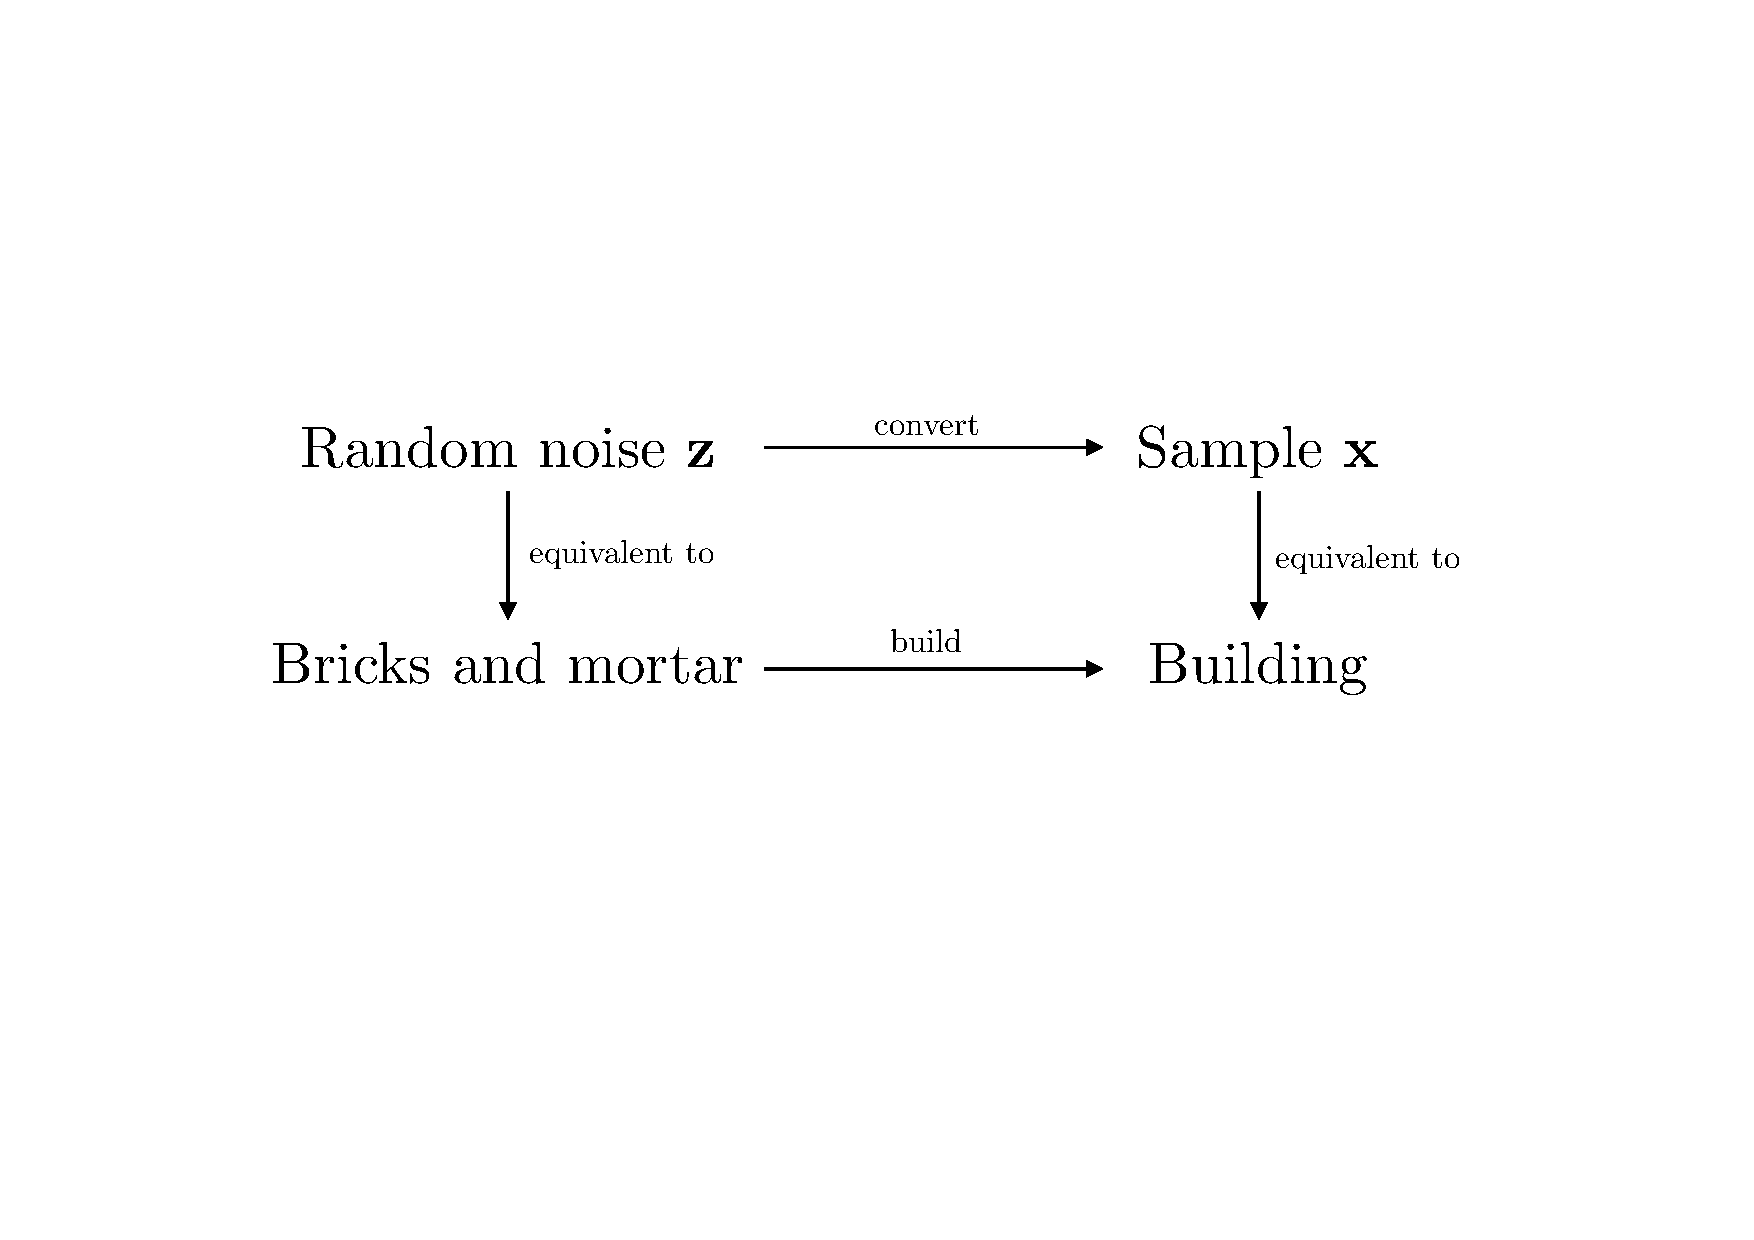
\includegraphics[width=0.5\linewidth]{loop.pdf}
    \caption{Building construction analogy to the DDPM model.}
    \label{fig:analogy}
\end{figure}

We can rethink of the process as a building process, where the noises $\bm{z}$ are the raw materials, in this case, the bricks and mortar, and the samples $\x$  are the final buildings being built. In this case, the generative model becomes the construction team. 

The reconstruction process is bound to be difficult, and this is why there are so many researches involved in the development of generative models. On the other hand, the demolition process is very easy. Considering a \textbf{step-wise process} that gradually demolishing a building into bricks, in this case, let $\x_0$ be the fully-constructed building (initial sample) and $\x_T$ being the fully deconstructed bricks (random noises). Assuming the demolition takes $T$ steps, then the whole demolition process can be written as 
\begin{equation}\label{eq:1.2}
    \x=\x_0\to\x_1\to\x_2\to\cdots \x_{T-1}\to \x_{T}=\bm{z}.
\end{equation}
Within this framework,\marginnote{\footnotesize{\textcolor{red}{It is important to take a note of this at this point, as this is a recurrent trick in the diffusion generative model that tries to learn the reverse construction process. This can be parameterised by any major NN architetures, including convolutional NN, transformer, graph and message-passing NNs for learning atomistic structures. In this regard, diffusion model has very little to do with the designs of the NN but more with the manipulations in the probability distributions of the data.}}} the difficulties in rebuilding a building is that, the jump from the raw materials $\x_T$ to the final building $\x_0$ is too large for a novelist to comprehend how this process can be achieved. However, if we have the intermediate states from the demolition processes $\x_1$, $\x_2$ till $\x_{T-1}$, and we know $\x_{t-1}\to\x_{t}$ represents one small demolition step, then why can't we utilise these information to learn the reverse process $\x_{t}\to\x_{t-1}$ to rebuild the building? This means that if we can learn the relationship between the two \textcolor{red}{$\bmu(\xt)=\xtm$}, then starting from $\x_{T}$, by repetitively applying $\x_{T-1}=\bmu(\x_{T})$,  $\x_{T-2}=\bmu(\x_{T-1})$ and so on, wouldn't we be able to rebuild the whole building $\x_0$?

\subsection{How should we demolish the building?}

Just like we need to eat our meals bite by bite, we also need to rebuild our buildings stepwise. The process of generation in DDPM is actually fully consistent with the the \textbf{analogy of ``demolition followed by reconstruction''} for DDPM. It is a process that first gradually deconstruct the data samples into random noises, then considers a reverse process which is carried out repetitively to (re)generated the (original) new samples. As mentioned before, this is why DDPM is more like a model of \textbf{progressive change} rather than a diffusion model.

More specifically, the demolition process in DDPM takes the following form:
\begin{equation}
    \label{eq:1.3}
    \xt=\alpha_t\x_{t-1}+\beta_t\bm{\varepsilon}_t,\quad\mbox{with}\quad\bm{\varepsilon}_t\sim \mathcal{N}(0,\bm{I}),
\end{equation}
in particular, $\alphat$ and $\betat>0$, $\alphat^2+\betat^2=1$. Usually, we chose $\betat\to0$, it represents how much damage we will make to the building during each step of the demolition process. The introduction of the \textbf{noise} $\et$ represents the destruction to the original signal. We can also think of it as the raw materials, such that in each step of the demolition process, we break $\xtm$ into $\alphat \xtm$ part of the original building plus $\betat\et$ part of the raw materials.

If we repeat the above process, then we have
\begin{align}
\xt&=\alphat\xtm+\betat\et\nonumber\\
&=\alphat\left(\alphatm\bm{x}_{t-2}+\betatm\bm{\varepsilon}_{t-1}\right)+\betat\et\nonumber\\
&=\cdots\nonumber\\
&=(\alphat\alphatm\cdots\alpha_1)\bm{x}_0+\textcolor{red}{(\alphat\alphatm\cdots\alpha_2)\beta_1\bm{\varepsilon}_1+(\alphat\cdots\alpha_3)\beta_2\bm{\varepsilon}_2+\cdots+\betat\et}. \marginnote{\textcolor{red}{\footnotesize{This part is the sum of multiple independent Gaussian noises.}}}\label{eq:1.4}
\end{align}
So why do we require the coefficients must satisfy the constraint $\alphat^2+\betat^2=1$? Let us try to answer this question. In \cref{eq:1.4}, the part that is highlighted in red represents the sum of multiple independent Gaussian noises with the mean of zero, and variances being $(\alphat\alphatm\cdots\alpha_2)\beta_1$, $(\alphat\cdots\alpha_3)\beta_2$, $\ldots$, $\alphat\betatm^2$ and $\betat^2$, respectively. Then, based on the superposition of Gaussians from the probability theory, the sum of Gaussians returns a new Gaussian, which, in the case is of mean zero and variance given by $(\alphat\alphatm\cdots\alpha_2)\beta_1+(\alphat\cdots\alpha_3)\beta_2+\cdots+\betat$. Providing that $\alphat^2+\betat^2=1$, it is not difficult to prove that 
\begin{equation}
    \label{eq:1.5}
(\alphat\alphatm\cdots\alpha_2)\beta_1+(\alphat\cdots\alpha_3)\beta_2+\cdots+\betat=1.
\end{equation}
This means that, effectively, we have \marginnote{\footnotesize{\textcolor{red}{Take note of the definitions $\baralphat=\prod_{i=1}^t\alpha_i$ and $\barbetat=\sqrt{1-\baralphat^2}$, which are commonly used in the diffusion models.}}}
\begin{equation}
    \label{eq:1.6}
\xt=\underbrace{(\alphat\cdots\alpha_1)}_{\equiv\textcolor{red}{\baralphat}}\bm{x}_0+\underbrace{\sqrt{1-(\alphat\cdots\alpha_1)^2}}_{\equiv\textcolor{red}{\barbetat}}\bar{\bm{\varepsilon}}_t,\qquad\bar{\bm{\varepsilon}}_t\sim\mathcal{N}(0,\bm{I}),
\end{equation}
which has now significantly simplified the computations of $\xt$. On the other hand, by choosing a suitable form of $\alphat$ in DDPM to ensure $\baralphat\approx0$ will guarantee that, after $T$ steps of demolitions, the entire building will be fully deconstructed into its raw materials $\bm{\varepsilon}$.

\subsection{How to rebuild the building?}

During the demolition process $\xtm\to\xt$, we can obtain many pairs of data $(\xtm,\xt)$, therefore, rebuilding is simply a process that learns a model to enable the reverse process $\xt\to\xtm$ to occur. Suppose this model is $\muxt$, then the most straightforward learning protocol is to minimise the Euclidean distance
\begin{equation}
    \label{eq:1.7}
    \|\muxt-\xtm\|_2^2.
\end{equation}
This simple formulation is actually very close to the final DDPM model. Here, we can refine it further. If we first rearrange \cref{eq:1.3} from the demolition process into a reconstructing one by making $\xtm$ the subject:
\begin{equation*}
    \xtm=\frac{1}{\alphat}\left(\xt-\betat\et\right),
\end{equation*}
this then inspires us to express the parameterised reconstruction process analogously as
\begin{equation}
    \label{eq:1.8}
    \muxt=\frac{1}{\alphat}\left(\xt-\betat\bm{\varepsilon}_\theta(\xt,t)\right),
\end{equation}
in which $\theta$ is the learnable parameter. Substituting \cref{eq:1.8} into the loss function \cref{eq:1.7}, we get
\begin{equation}
    \label{eq:1.9}
    \|\muxt-\xtm\|_2^2=\frac{\betat^2}{\alphat^2}\|\et-\bm{\varepsilon}_\theta(\xt,t)\|_2^2.
\end{equation}
Here, $\betat^2/\alphat^2$ represents the weight of the loss function, which we can ignore it for the time being. Substituting  \cref{eq:1.3} and \cref{eq:1.6} for the expression of $\xt$:
\begin{equation}
    \label{eq:1.10}    \xt=\alphat\xtm+\betat\et=\alphat(\alphatmbar\bm{x}_0+\betatmbar\bar{\bm{\varepsilon}}_{t-1})+\betat\et=\alphat\bm{x}_0+\alphat\betatmbar\bar{\bm{\varepsilon}}_{t-1}+\betat\et,
\end{equation}
from which we arrive at a new form of the loss function:
\begin{equation}
    \label{eq:1.11}
    \|\et-\bm{\varepsilon}_\theta(\alphat\bm{x}_0+\alphat\betatmbar\bar{\bm{\varepsilon}}_{t-1}+\betat\et,t) \|_2^2.
\end{equation}
Some readers may wonder why, in \cref{eq:1.10}, we have to go back on step to $t-1$, rather than just go from $t$ to 0 directly? \marginnote{\footnotesize{This process of stepping back one more step will occur recurrently in many derivations in the subsequent chapters.}}
The answer is that, since  we already sampled $\et$ in \cref{eq:1.9}, and $\bar{\bm{\varepsilon}}_t$ is not independent from $\et$, we cannot sample $\bar{\bm{\varepsilon}}_t$ completely as an independent variable, in which case we end up minimising towards a target that is sample dependent.

\subsection{Reducing the square error}
In principle, we could train DDPM directly using the loss function \cref{eq:1.11}. But in real practice, this is not very tractable, which can lead to slow convergence. This is because \cref{eq:1.11} involves \textbf{four} random variables that can only be obtained through samplings:
\begin{enumerate}
    \item A random sample $\bm{x}_0$ from the inputs.
    \item Sample $\bar{\bm{\varepsilon}}_{t-1}$ and $\bar{\bm{\varepsilon}}_{t}$ from a normal distribution $\mathcal{N}(0,\bm{I})$, giving extra two variables.
    \item Choosing a $t$ from 1 to $T$.
\end{enumerate}
The more we need to sample, the more challenge it is to compute the loss function accurately! Fortunately, this problem can be partially mitigated by combining $\et$ and $\bar{\bm{\varepsilon}}_{t-1}$ into a single random variable sampled from a normal distribution using the integration trick. Because the product of two normal distributions is still a normal distribution, so we have $\alphat\betatmbar\bar{\bm{\varepsilon}}_{t-1}+\betat\et$ is equivalent to $\betatbar\bm{\varepsilon}|\bm{\varepsilon}\sim\mathcal{N}(0,I)$. Equally, we have \textcolor{blue}{$\betat\bar{\bm{\varepsilon}}_{t-1}-\alphat\betatmbar\et$ is equivalent to $\betatbar\bm{w}|\bm{w}\sim\mathcal{N}(0,I)$}.\marginnote{\footnotesize{\textcolor{blue}{Not quite sure where this comes from?}}} Furthermore, it can be proven that $\mathbb{E}[\bm{\varepsilon}\bm{w}^T]=0$, so they are two independent normal distributions. With this, we can express $\et$ with $\bm{\varepsilon}$ and $\bm{w}$:
\begin{equation}
    \label{eq:1.12}
    \et=\frac{(\betat\bm{\varepsilon}-\alphat\betatmbar\bm{w})\betatbar}{\betat^2+\alphat^2\betatmbar^2}=\frac{\betat\bm{\varepsilon}-\alphat\betatmbar\bm{w}}{\betatbar}.
\end{equation}
Substitute \cref{eq:1.12} into \cref{eq:1.11}, we get
\begin{align}
    &\mathbb{E}_{\bar{\bm{\varepsilon}}_{t-1},\et\sim\mathcal{N}(0,\bm{I})}\left[\left\| \et-\bm{\varepsilon}_\theta(\alphat\bm{x}_0+\alphat\betatmbar\bar{\bm{\varepsilon}}_{t-1}+\betat\et,t) \right\|_2^2\right]\nonumber\\
    &=\mathbb{E}_{\bm{w},\bm{\varepsilon}\sim\mathcal{N}(0,\bm{I})}\left[\left\| \frac{\betat\bm{\varepsilon}-\alphat\betatmbar\bm{w}}{\betatbar}-\bm{\varepsilon}_\theta (\alphatbar\bm{x}_0+\betatbar\bm{\varepsilon},t)   \right\|_2^2 \right]. \label{eq:1.13}
\end{align}
Note that the loss function is quadratic in $\bm{w}$, which we can expand the square and then determine the expectation value, this gives,
\begin{equation}
    \label{eq:1.14}
    \frac{\betat^2}{\betatbar^2}\mathbb{E}_{\bm{\varepsilon}\sim\mathcal{N}(0,\bm{I})}\left[\left\| \bm{\varepsilon}-\frac{\betatbar}{\betat}\bm{\varepsilon}_\theta (\alphatbar\bm{x}_0+\betatbar\bm{\varepsilon},t)   \right\|_2^2 \right]+\mathcal{C}.
\end{equation}
Ignoring the weight and constant again, we arrive at:\marginnote{\footnotesize{\textcolor{red}{This basically says, we must first sample a noise from the normal distribution $\mathcal{N}(0,\bm{I})$, from which we can generate the noisy sample $\xt=\alphatbar\bm{x}_0+\betatbar\bm{\varepsilon}$. Then we plug this $\xt$ into the denoising network $\bm{\varepsilon}_\theta(\xt)$ to recover $\et$. This expression is equivalent to the results\cite{luo2022understanding} derived using KL divergence between the destruction and regeneration process: $\argmin_\theta\mathcal{D}_{KL}(q(\xtm|\xt,\bm{x}_0)$ $\|p(\xtm|\xt))$ from evidence lower bound, which upon further reparameterisation, gives the following expression for the KL divergence: $\frac{(1-\alphat)^2}{2\sigma_q^2(t)}\frac{\|\bm{\varepsilon}_0-\hat{\bm{\varepsilon}}_\theta(\bm{x},t)\|_2^2}{(1-\alphatbar)\alphat}$.}}}
\textcolor{red}{
\begin{equation}\label{eq:1.15}
    \mathbb{E}_{\bm{\varepsilon}\sim\mathcal{N}(0,\bm{I})}\left[\left\| \bm{\varepsilon}-\frac{\betatbar}{\betat}\bm{\varepsilon}_\theta (\alphatbar\bm{x}_0+\betatbar\bm{\varepsilon},t)   \right\|_2^2 \right],
\end{equation}}
which is the final form of the lost function for DDPM.

\subsection{Regressive generations}
Above, we have clarified the training procedures for DDPM. The derivation is a bit lengthy and not immediately trivial. While it is not easy to understand, it is not totally difficult either, since it has not applied the mathematical tools that are needed in the traditional diffusion models, but only an analogous model of building demolition and reconstruction plus some basic knowledge in the probability theory. As such, this newly formulated diffusion generated model, as represented by DDPM, is not as mathematically complicated as one may think. 

After the model is being trained, we can perform samplings to generate new samples. Starting from a random noise $\bm{x}_T\sim\mathcal{N}(0,\bm{I})$, and repeat the process for $T$ steps according to \cref{eq:1.8}:
\begin{equation}
    \label{eq:1.16}
    \xtm=\frac{1}{\alphat}(\xt-\betat\bm{\varepsilon}_\theta(\xt,t)).
\end{equation}
This corresponds to the \textbf{greedy search} in VAE. For random sampling, we can add an additional noise term:
\begin{equation}
    \label{eq:1.17}
    \xtm=\frac{1}{\alphat}(\xt-\betat\bm{\varepsilon}_\theta(\xt,t))+\sigma_t \bm{z}\qquad \bm{z}\sim\mathcal{N}(0,\bm{I}).
\end{equation}
In practice, \textcolor{red}{we can keep $\betat=\sigma_t$}, i.e., the variances are the same for both the forward and reverse diffusions.

It should be noted that the sampling process in DDPM is different from the one performed with Langevin equation. In DDPM, each sampling process starts from a new random noise, and is iterated for $T$ steps to generate a new sample. On the other hand, Langevin sampling starts from a single random point and iterates definitively. In principle, all samples can be generated through infinite iterations. Therefore, although DDPM shares similarity with the Langevin sampling, they are fundamentally different models.

\subsection{Hyperparameter settings}
In DDPM, the upper limit $T$ is usually set to 1000, which is much larger than what people usually expect. Why such a large value is necessary? In the original publication, the following function is used to set $\alphat$:
\begin{equation}
    \label{eq:1.18}
    \alphat=\sqrt{1-\frac{0.02t}{T}},
\end{equation}
which is a monotonically decreasing function. Why such a choice is also necessary?

The above two questions are inter-dependent, and is related to the nature of the data. When the Euclidean distance is used for constructing the loss function, experience of image reconstructions using VAE shows that, only when the input and output images are sufficiently close to each other, we can generate new images of higher quality. Thus, using large time can make sure the input and output in each time step are sufficiently similar to each other, reducing the blurring effects from using the Euclidean distance in the loss function. 

A similar reason applies to  the choice of a monotonically decreasing function for $\alphat$. When $t$ is small, $\xt$ is close to the real image, so we need to decrease the distance between $\xtm$ and $\xt$, making it more suitable to apply the Euclidean distance in \cref{eq:1.7}. This gives large $\alphat$. When $t$ is very large, $xt$ becomes very close to a true Gaussian noise, which can be modelled with the Euclidean distance, thus we can increase the distance between $\xtm$ and $\xt$ with smaller $\alphat$. Can we use a large $\alphat$ throughout the forward process then? In principle the answer is yes, but we need to increase $T$. Recall that when we derived \cref{eq:1.6}, we wanted $\bar{\alpha}_T\approx0$, which we can evaluate
\begin{equation}
    \label{eq:1.19}
    \log\bar{\alpha}_T=\frac{1}{2}\sum_{t=1}^T \log \left( 1-\frac{0.02t}{T}\right) < \frac{1}{2}\sum_{t=1}^T \log \left(-\frac{0.02t}{T}\right)=-0.005(T+1)
\end{equation}
With $T=1000$, $\bar{\alpha}_T\approx 10^{-5}$, which is nearly zero as we wished. As a result, if we want to use a large $\alpha_t$ throughout, then we will have to increase $T$.

Finally, note that in the loss function [\cref{eq:1.15}, $\bm{\varepsilon}_\theta(\alphatbar\bm{x}_0+\betatbar\bm{\varepsilon},t)$], the time variable $t$ has been explicitly included. This is because, at different $t$, we are dealing with data of different noise levels. Therefore, \textbf{we are required to have $T$ different reconstruction models}, meaning \textbf{$T$ is also a model hyperparameter}.
\section{DDPM=Autoregressive VAE}
\marginnote{\footnotesize{Original blog post see \url{https://www.spaces.ac.cn/archives/9152}}}

In \cref{section:DDPM_1}, we had established an analogy for the diffusion generative model DDPM, in which we described it as the process of demolition followed by reconstruction. Based on this analogy, we have completed a particular form of the mathematical derivations for the theoretical foundation of DDPM. We also pointed out that, fundamentally, DDPM is not the traditional diffusion model, but more like a VAE. In fact, in the seminal paper for DDPM\cite{ho2020denoising}, it was derived based on the VAE framework. Therefore, in this section, we will reintroduce the DDPM diffusion model based on the framework of VAE.

\subsection{Solving the problem step-wise}

In the standard formulation of the VAE, \marginnote{\footnotesize{In the language of VAE,  $\bm{z}$ is usually referred to as the \textit{latent variable}.}} both the encoding and generative processes are completed in a single step:
\begin{equation}
    \label{eq:2.1}
    \mbox{ENCODER: }\quad \bm{x}\to\bm{z};\quad\mbox{GENERATION: }\quad\bm{z}\to\bm{x}.
\end{equation}
In this case, we only need to deal with three data distributions: the \textbf{encoding distribution} $p(\bm{z}|\bm{x})$, the \textbf{generative distribution} $q(\bm{x}|\bm{z})$, and the prior distribution $q(\bm{z})$. The advantage behind such a formulation is its simplicity. There also exists a simple projective relationship between the sample $\bm{x}$ and the latent variable $\bm{z}$, such that we can train and obtain both the encoder and the decoder (generator) simultaneously. it also allows us to manipulate the data in the latent space. However, VAE also has its notable limitations. Since all three distributions are usually modelled as the normal distributions, it has resulted in the limited expressive capability of the VAE model. 

To overcome this limitation, DDPM breaks these processes into multiple steps:
\begin{align}
    \mbox{ENCODER: }\quad&\bm{x}=\bm{x}_0\to\bm{x}_1\to\bm{x}_2\to\cdots\to\bm{x}_{T-1}\to\bm{x}_{T}=\bm{z}\nonumber\\
    \mbox{DECODER: }\quad &\bm{z}=\bm{x}_{T}\to\bm{x}_{T-1}\to\bm{x}_{T-2}\to\cdots\to\bm{x}_1\to\bm{x}_{0}=\bm{x}.\label{eq:2.2}
\end{align}
In this way, every transition probability $p(\xt|\xtm)$ or $q(\xtm|\xt)$  is only responsible for making a small change to the sample by the model. One may ask, if both $p$ and $q$ are normal distributions, why this alternative model will work better than the single-stepped one [\cref{eq:2.1}]? This is because, \emph{Gaussian distributions work better in approximating small incremental changes}, which is similar to approximating a curve with linear relationship that will only work within a small region of $\Delta\bm{x}$. As such, theoretically, the formulation proposed in \cref{eq:2.2} is able to improve the performance of a single-shot VAE.

\subsection{The joint KL divergence}
To arrive at a step-wise formulation for VAE, we have \textcolor{red}{$p(\xt|\xtm)$} for every encoding step and \textcolor{red}{$q(\xtm|\xt)$} for every generation step.
\marginnote{\footnotesize{\textcolor{red}{In the following derivations, the convention behind VAE will be adopted, in which we will use $p$ for the transition probability of the forward (encoding) process and $q$ for the backward (decoding) process, which is \textbf{opposite} to the notations used in the DDPM literatures!}}} This allows us to write down the \textbf{joint probability distributions}:
\begin{align}
p(\bm{x}_{0},\bm{x}_1,\bm{x}_2,\ldots,\bm{x}_T)&=p(\bm{x}_T|\bm{x}_{T-1})\cdots p(\bm{x}_2|\bm{x}_1)p(\bm{x}_1|\bm{x}_0)\tilde{p}(\bm{x}_{0})\nonumber\\
q(\bm{x}_{0},\bm{x}_1,\bm{x}_2,\ldots,\bm{x}_T)&=q(\bm{x}_0|\bm{x}_1)\cdots q(\bm{x}_{T-2}|\bm{x}_{T-1})q(\bm{x}_{T-1}|\bm{x}_{T})q(\bm{x}_T). \label{eq:2.3}
\end{align}
Here, $\bm{x}_0$ represents the input samples, thus $\tilde{p}(\bm{x}_0)$ represents the sample distribution, whereas $q(\bm{x}_T)$ is the prior distribution, as $\bm{x}_T$ is the final encoded sample. The rest probability distributions of the type $p(\xt|\xtm)$ and $q(\xtm|\xt)$ represent each small step in the encoding and generating processes, respectively.

The simplest way to understand VAE, is to minimise the KL divergence between the joint probability distributions, which is equally applicable to DDPM:
\begin{equation}
    \label{eq:2.4}
    D_{KL}(p\|q)=\int p(\bm{x}_T|\bm{x}_{T-1})\cdots p(\bm{x}_1|\bm{x}_0)\tilde{p}(\bm{x}_{0}) \log\frac{p(\bm{x}_T|\bm{x}_{T-1})\cdots p(\bm{x}_1|\bm{x}_0)\tilde{p}(\bm{x}_{0})}{q(\bm{x}_0|\bm{x}_1)\cdots q(\bm{x}_{T-1}|\bm{x}_{T})q(\bm{x}_T)}d\bm{x}_0\cdots d\bm{x}_T.
\end{equation}
This is, therefore, the optimisation target for DDPM. What is left is to consolidate the forms of $p(\xt|\xtm)$ and $q(\xtm|\xt)$ to simplify \cref{eq:2.4} further, making it possible to be computed numerically.

\subsection{Divide-and-conquer}
First of all, DDPM is only interested in the generating part of the process, therefore, in the encoder process, every step is modelled as a simple normal distribution:
\begin{equation*}
    p(\xt|\xtm)=\mathcal{N}(\xt;\alphat\xtm,\betat^2\bm{I}).\marginnote{\footnotesize{This is an alternative way of writing \cref{eq:1.3}}}
\end{equation*}
This is much simpler than the VAE,  the medium and variance of which are both learnt by a neural network. Here, the medium is basically $\xtm$ that is multiplied by a \emph{scalar} $\alphat$. Hence, DDPM has completely abandoned the capability to encode the data, and only established a generative model. The transition probability for the generating process $q(\xtm|\xt)$ has now been formulated as a learnable model $\mathcal{N}(\xtm;\muxt,\sigma_t^2\bm{I})$. Here, \textbf{$\alphat$, $\betat$ and $\sigma_t$ are all not learnables but parameterised.} Hence, $\muxt$ is the only trainable object in the entire diffusion model.

Since $p$ is not parameterised, the integration in \cref{eq:2.4} that involves purely the $p$ distributions can be factored out as a constant. This makes \cref{eq:2.4} become equivalent to
\begin{align}
    &\quad -\int p(\bm{x}_T|\bm{x}_{T-1})\cdots p(\bm{x}_1|\bm{x}_0)\tilde{p}(\bm{x}_{0})  \underbrace{\textcolor{red}{\log[q(\bm{x}_0|\bm{x}_1)\cdots q(\bm{x}_{T-1}|\bm{x}_T)q(\bm{x}_{T})]}}_{\mbox{\textcolor{red}{make this into a summation}}}  d\bm{x}_0\cdots d\bm{x}_T \nonumber\\
    &=-\int p(\bm{x}_T|\bm{x}_{T-1})\cdots p(\bm{x}_1|\bm{x}_0)\tilde{p}(\bm{x}_{0}) \textcolor{red}{\left[\log q(\bm{x}_T)+\sum_{t=1}^T\log q(\xtm|\xt)\right]}  d\bm{x}_0\cdots d\bm{x}_T. \label{eq:2.5}
\end{align}
Since $q(\bm{x}_T)$ is usually modelled as a normal distribution, it is also parameter-free. As such, we only need to compute \emph{every term} of the form
\begin{align}
\marginnote{\footnotesize{\textcolor{red}{This integral ismaximally dependent up to $\xt$, so all the integrations from $\bm{x}_{t+1}$ to $\bm{x}_T$ gives unity, allowing us to remove some terms involving $p$.}}}
    &\quad -\int \underbrace{p(\bm{x}_T|\bm{x}_{T-1})\cdots p(\bm{x}_1|\bm{x}_0)\tilde{p}(\bm{x}_{0})}_{T+1\mbox{ terms}} \textcolor{red}{\log q(\xtm|\xt)} d\bm{x}_0\cdots d\bm{x}_T\nonumber\\
    &=-\int \underbrace{p(\xt|\xtm)\cdots p(\bm{x}_1|\bm{x}_0)\tilde{p}(\bm{x}_{0})}_{t+1\mbox{ terms}}\log q(\xtm|\xt)d\bm{x}_0\cdots d\bm{x}_{\textcolor{red}{t}}\nonumber\\
\marginnote{\footnotesize{\textcolor{red}{Similarly, the integral is also independent from $x_1$, $\ldots$, $x_{t-2}$.}}}
&=-\int p(\xt|\xtm)p(\xtm|\bm{x}_0)\tilde{p}(\bm{x}_{0})\log q(\xtm|\xt)d\bm{x}_0 d\bm{x}_{t-1}\bm{x}_t. 
\end{align}

\subsection{Reconstructing the diffusion model}
What follows from here is basically the same as discussed in \cref{chap_1:rebuild}:
\begin{myquote}
\begin{enumerate}
\item Remove all the constants that are irrelevant to the optimisation problem, this left us with the term $-\log q(\xtm|\xt)$ which gives the term $\frac{1}{2\sigma_t^2}\|\xtm-\muxt\|_2^2$ in the target function for optimisation.
\item The transition probability $p(\xtm|\bm{x}_0)$ can be equivalently written as $\xtm=\alphatmbar\bm{x}_0+\betatmbar\bar{\bm{\varepsilon}}_{t-1}$, similarly $p(\xt|\xtm)$ implies $\xt=\alphat\xtm+\betat\et$, in which $\bar{\bm{\varepsilon}}_{t-1}$ and $\et\sim\mathcal{N}(0,\bm{I})$.
\item From $\xtm=\frac{1}{\alphat}(\xt-\betat\et)$, it inspires us to parameterise $\muxt$ as $\muxt=\frac{1}{\alphat}(\xt-\betat\bm{\varepsilon}_\theta(\xt,t))$.
\end{enumerate}
\end{myquote}
Equipped with these transformations, the target function for optimisation can be rewritten in the following form:\marginnote{\footnotesize{\textcolor{red}{This is equivalent to \cref{eq:1.11}.}}}
\begin{equation}
    \label{eq:2.7}
    \frac{\betat^2}{\alphat^2\sigmat^2}\mathbb{E}_{\bar{\bm{\varepsilon}}_{t-1},\et\sim\normdist,\bm{x}_{0}\sim\tilde{p}(\bm{x}_{0})}\left[\left\| \et-\es (\alphatbar \bm{x}_0+\alphat\betatmbar\etm +\betat\et,t)  \right\|_2^2\right].
\end{equation}
This is followed by the trick of changing the variables applied in \cref{sect1:reduce_error}, which gives\marginnote{\footnotesize{\textcolor{red}{This is equivalent to \cref{eq:1.15}.}}}
\begin{equation}
    \label{eq:2.8}
    \frac{\betat^4}{\alphat^2\sigmat^4}\mathbb{E}_{\bm{\varepsilon}\sim\normdist,\bm{x}_{0}\sim\tilde{p}(\bm{x}_{0})}\left[\left\| \et-\frac{\betatbar}{\betat}\es(\alphatbar\bm{x}_0 +\betatbar\bm{\varepsilon},t)  \right\|_2^2\right]
\end{equation}
This leads to the loss function for DDPM. \textbf{As tested in the original paper, the model performance is even better if we drop the coefficient $\frac{\betat^4}{\alphat^2\sigmat^4}$ in the numerical implementation. } The above derivation starts from the loss function for VAE and sequentially simplifies the multivariant integral [\cref{eq:2.5}]. Although the derivation is longer, it is logically tractable. In comparison to the original DDPM paper\cite{ho2020denoising}, where a conditional probability $q(\xtm|\xt,\x_0)$ was introduced which then split the terms that were subsequently cancelled out. This original derivation came somehow `out of the blue', which may not be easily understood by many readers.

\subsection{Hyperparameter settings}

Now we move on to discuss the choice of the hyperparameters $\alphat$, $\betat$ and $\sigmat$. For $p(\xt|\xtm)$, it is conventional to set $\alphat^2+\betat^2=1$, which already allows us to reduce the number of hyperparameters by half, and helps to simplify the expressions. This has already been discussed in \cref{section:DDPM_1}. From the superposition of normal distributions, we have the following formula one-shot sampling:
\begin{equation}
    \label{eq:2.9}
    p(\xt|\x_0)=\int p(\xt|\xtm)\cdots p(\x_1|\x_0)d\xt d\xtm\cdots d\x_1=\mathcal{N}(\xt;\alphatbar\x_0,\betatbar^2\bm{I}),
\end{equation}
where $\alphatbar=\alpha_1\alpha_2\cdots\alphat$, and $\betatbar=\sqrt{1-\alphatbar^2}$.

So what inspires us to set $\alphat^2+\betat^2=1$? The choice of $\mathcal{N}(\xt;\alphatbar\x_0,\betatbar^2\bm{I})$ means we have $\xt=\alphat\x_{t-1}+\betat\et$ with $\et\sim\normdist$, then it would require $\alphat^2+\betat^2=1$ based on the normalisation condition for the linear combinations of normal distributions.

As mentioned before, we usually represent $q(\x_T)$ as a standard normal distribution $\mathcal{N}(\x_T;0,\bm{I})$, and the training goal is to minimise the KL divergence of the two joint probability distributions, i.e. $p=q$. This means that the marginal distributions should also equal each other:
\begin{align}
    q(\x_T)&=\int p(\x_T|\x_{T-1}) p(\x_{T-1}|\x_{T-2})\cdots p(\x_1|\x_0)\tilde{p}(\x_0)d\x_0 d\x_1 \cdots d\x_{T-1} \nonumber\\
    &=\int p(\x_T|\x_0)\tilde{p}(\x_0) d\x_0. \label{eq:2.10}
\end{align}
In general, the sample distribution is arbitrary, such that the only way to make \cref{eq:2.10} hold is to equate $p(\x_T|\x_0)$ to become $q(\x_T)$ [Note that the integral in  \cref{eq:2.10} is independent of $\x_T$!]. \textbf{It means to evolve $\tilde{p}(\x_0)$ into a Gaussian distribution that is independent from $\x_0$.} Recall that $q(\x_T)\sim\mathcal{N}(\xt;\alphatbar\x_0,\betatbar^2\bm{I})$, this would require $\alphatbar \approx 0$ when $t\to T$. More discussions on the choice of $\alphat$ can be referred back to \cref{chap_1:rebuild}.

For $\sigmat$, \marginnote{\footnotesize{\textcolor{red}{$\sigmat$ comes from the definition of $q(\xtm|\xt)$, which we formulated it as a learnable distribution $\mathcal{N}(\xtm;\muxt,\sigmat^2\bm{I})$, this is needed for the reverse sampling process.}}} in theory, different sample distributions $
\tilde{p}(\x_0)$ will lead to a different optimised $\sigmat$. However, we do not really want to train the variance as an extra parameter. In this case, we can choose two special examples.
\begin{myquote}
    \begin{enumerate}
        \item Assume there is only one training sample, $\x_{*}$. In this case, we have $\tilde{p}(\x_0)=\delta(\x-\x_{*})$, the Dirac distribution. This will give an optimum value of $\sigma_t=\betatmbar\betat/\betatbar$.
        \item Assume $\tilde{p}(\x_0)\sim\normdist$, then the optimum $\sigmat=\betat$.
    \end{enumerate}
\end{myquote}
Both choices lead to comparable performances in practice. The proofs of these results are rather complicated, which will be reserved for the discussions in the next section.
%\section{DDPM=Bayes Plus Denoising}
\marginnote{\footnotesize{Original blog post see \url{https://www.spaces.ac.cn/archives/9164}}}

In the previous two sections, we have provided two different mathematical derivations for DDPM. The first one is based on an analogous comparison to the building of a house, which is easy to understand, but difficult to be extended theoretically. In the second approach, we draw our conclusions from  the framework of autoregressive variational autoencoder. Although theoretically more robust,. it is rather formal and lack of inspiration for  further improvements. In this section, we will give another derivation of the DDPM, which applies the Bayes' rule to simplify the computations. The derivation contains more reasoning,  which makes it more inspirational. Such derivation also has a deeper relationship with the DDIM,\marginnote{\footnotesize{\textcolor{red}{Diffusion Denoising Implicit Model}}} which is to be discussed in the next section.

\subsection{Recap on the model setup}
Recall that in the DDPM models, the forward process is modelled as a process of progressive transformation:
\begin{equation}
    \label{eq:3.1}
    \bm{x}=\bm{x}_0\to\bm{x}_1\to\bm{x}_2\to\cdots\to\bm{x}_{T-1}\to\bm{x}_{T}=\bm{z}
\end{equation}
in which the process gradually adds noise to the sample $\x$ and transform it into a pure noise $\bm{z}$, whereas the reverse process gradually denoises $\bm{z}$ to recover the sample data $\x$. This reverse process is the generative model that we aim to build.

The forward process is simple to achieve, in which every step is given by
\begin{equation}
    \label{eq:3.2}
    \xt=\alphat\xtm+\betat\et\qquad \et\sim\normdist,
\end{equation}
which can be equivalently written as $p(\xt|\xtm)=\mathcal{N}(\xt;\alphat\xtm,\betat^2\bm{I})$. Under the constraint of $\alphat^2+\betat^2=1$, we have the following:
\begin{align}
    \xt&=\alphat\xtm+\betat\et \nonumber\\
    &=\alphat(\alphatm\x_{t-2}+\betatm \etm)    +\betat\et \nonumber\\
    &=\cdots\nonumber\\
    &= (\alphat\cdots\alpha_1)\x_0+\underbrace{(\alphat\cdots\alpha_2)\beta_1\bm{\varepsilon}_1+(\alphat\cdots\alpha_3)\beta_2\bm{\varepsilon}_2+\cdots+\alphat\betatm\etm+\betat\et}_{\sim\mathcal{N}(0,(1-\alphat^2\cdots\alpha_1^2)\bm{I})}
    \label{eq:3.3}
\end{align}
From which we have $p(\xt|\x_0)=\mathcal{N}(\xt;\alphatbar\x_0,\betatbar^2\bm{I})$ with $\alphatbar=\alpha_1\cdots\alphat$ and $\betatbar=\sqrt{1-\alphatbar^2}$. What DDPM is trying to achieve, is to figure out how to obtain \textcolor{red}{$p(\xtm|\xt)$} for the reverse generation process using the information above. With this, we could start from any arbitrary $\bm{z}=\x_T$, and through sampling $\x_{T-1}$, $\x_{T-2}$, $\ldots$, $\x_1$ stepwise, we could eventually generate a new sample $\x=\x_0$.

\subsection{Using the Bayes' theorem} \marginnote{\footnotesize{\textcolor{red}{As such, in what follows, we will focus on deriving expressions for $p(\xtm|\xt)$}}}

According to the Bayes' theorem, we have, in this case
\begin{equation}
    \label{eq:3.4}
    p(\xtm|\xt)=\frac{p(\xt|\xtm)p(\xtm)}{p(\xt)}.
\end{equation}
However, we do not know what $p(\xtm)$ and $p(\x)$ look like, so we cannot move further from this expression. However, we know that these distributions are tractable once they are conditioned on the input $\x_0$. In this case, we have
\begin{equation}
    \label{eq:3.5}
    p(\xtm|\xt,\textcolor{red}{\x_0})=\frac{p(\xt|\xtm)p(\xtm|\textcolor{red}{\x_0})}{p(\xt|\textcolor{red}{\x_0})}.
\end{equation}
Since we know the expressions for $p(\xt|\xtm)$, $p(\xtm|\x_0)$ and $p(\xt|\x_0)$ (the latter two from one-shot sampling), \cref{eq:3.5} can be simplified into:
\textcolor{red}{
\begin{equation}
    \label{eq:3.6}
    p(\xtm|\xt,\x_0)=\mathcal{N}\left(\xtm; \frac{\alphat\betatmbar^2}{\betatbar^2}\xt+\frac{\alphatmbar\betat^2}{\betatbar^2}\x_0,\frac{\betatmbar^2\betat^2}{\betatbar^2}\bm{I}  \right).
\end{equation}
}
\begin{myquote}
\footnotesize{
To prove \cref{eq:3.6}, note that the exponent in \cref{eq:3.5}, ignoring the factor $\frac{1}{2}$, is
\begin{equation}\label{eq:3.7}
    \frac{\|\xt-\alphat\xtm\|_2^2}{\betat^2}+ \frac{\|\xtm-\alphatmbar\x_0\|_2^2}{\betatmbar^2} -  \frac{\|\xt-\alphatbar\x_0\|_2^2}{\betatbar^2}.
\end{equation}
This expression is quadratic in $\xtm$, so the finally distribution must also be a normal distribution. This means that we only need to determine the corresponding mean and variance. It can be shown that the coefficient for the $\|\xtm\|_2^2$ term is
\begin{equation}
    \label{eq:3.8}
    \frac{\alphat^2}{\betat^2}+\frac{1}{\betatmbar^2}=\frac{\alphat^2\betatmbar^2+\betat^2}{\betat^2\betatmbar^2}=\frac{\alphat^2(1-\alphatmbar^2)+(1-\alphat^2)}{\betat^2\betatmbar^2}=\frac{1-\alphatbar^2}{\betat^2\betatmbar^2}=\frac{\betatbar^2}{\betat^2\betatmbar^2}
\end{equation}
This means that the final exponent must be of the form $\frac{\betatbar^2}{\betat^2\betatmbar^2}\|\xtm-\tilde{\bm{\mu}}(\xt,\x_0)\|_2^2$, such that the covariance matrix is $\frac{\betat^2\betatmbar^2}{\betatbar^2}\bm{I}$. On the other hand, taking out the linear term in $\xtm$, the coefficient is $-2\left(\frac{\alphat}{\betat}\xt+\frac{\alphatmbar}{\betatmbar^2}\x_0\right)$, which, upon dividing by $-\frac{2\betat^2}{\betatmbar^2\betat^2}$, we get the following:
\begin{equation}
    \label{eq:3.9}
    \tilde{\bm{\mu}}(\xt,\x_0)= \frac{\alphat\betatmbar^2}{\betatbar}\xt+\frac{\alphatmbar\betat^2}{\betatbar^2}\x_0.
\end{equation}
By now, we have acquired all the information we need for the transition probability $p(\xtm|\xt,\x_0)$.
}
\end{myquote}

\subsection{The denoising process}
Although we now have an expression for  $p(\xtm|\xt,\x_0)$, this is not the final answer that we want. This is because ultimately we would like to predict $\xtm$ from $\xt$ that is independent from $\x_0$. If, on the other hand, we can predict $\x_0$ from $\xt$, then we would be able to estimate $\x_0$ in $p(\xtm|\xt,\x_0)$ and make it only dependent upon $\xt$. This can be achieved by letting $\x_0=\mubarxt$ as a learnable, with a loss function of $\|\x_0-\mubarxt\|_2^2$. After the model has been trained, we can write
\begin{equation}
    \label{eq:3.10}
    p(\xtm|\xt,\x_0)\approx p(\xtm|\xt,\x_0=\mubarxt)=\mathcal{N}\left(\xtm; \frac{\alphat\betatmbar^2}{\betatbar^2}\xt+\frac{\alphatmbar\betat^2}{\betatbar^2}\mubarxt,\frac{\betatmbar^2\betat^2}{\betatbar^2}\bm{I}  \right).
\end{equation}
In the expression $\|\x_0-\mubarxt\|_2^2$, $\x_0$ represents the original data, $\xt$ is the noised data. Hence, we are training a denoising model! This is the meaning of the first D in DDPM.

More specifically, $p(\xt|\x_0)=\mathcal{N}(\xt;\alphatbar\x_0,\betatbar^2\bm{I})$, which means $\xt=\alphatbar\x_0+\betatbar\bm{\varepsilon}$ with $\bm{\varepsilon}\sim\mathcal{N}(0,\bm{I})$, or equivalently, $\x_0=\frac{1}{\alphatbar}(\xt-\betatbar\bm{\varepsilon})$. This inspires us to parameterise $\mubarxt$ in the form of 
\begin{equation}
    \label{eq:3.11}
    \mubarxt=\frac{1}{\alphatbar}(\xt-\betatbar\es(\xt,t)).
\end{equation}
In this case, the loss function for training $\mubarxt$ becomes
\begin{equation}
    \label{eq:3.12}
    \|\x_0-\mubarxt\|_2^2=\frac{\betatbar^2}{\alphatbar^2}\|\bm{\varepsilon}- \betatbar\es( \alphatbar \x_0+\betatbar\bm{\varepsilon}  ,t) \|_2^2.
\end{equation}
Upon ignoring the coefficient $\betatbar^2/\alphatbar^2$, we thus recovered the loss function in the original DDPM paper. It can be seen that the derivation here from $\xt$ to $\xtm$ is more straight forward, which avoids the manipulations of integrals as done in the previous section. Now we can substitute \cref{eq:3.11} back into  \cref{eq:3.10} and simplify, which lead to
\textcolor{red}{
\begin{equation}
    \label{eq:3.13}
    p(\xtm|\xt,\x_0)\approx p(\xtm|\xt,\x_0=\mubarxt)=\mathcal{N}\left(\xtm; \frac{1}{\alphat}\left(\xt-\frac{\betat^2}{\betatbar} \es(\xt,t)\right),\frac{\betatmbar^2\betat^2}{\betatbar^2}\bm{I}  \right).
\end{equation}}
Once trained, this will be the probability distribution that will be used for the reverse sampling process. 
\begin{myquote}
    \footnotesize{
    To derive this result, note the following:
\begin{equation*}
    \frac{\alphatmbar\betat^2}{\betatbar^2}\frac{1}{\alphatbar}(\xt-\betatbar\es(\xt,t)) = \frac{\betat^2}{\betatbar^2\alphat}\xt- \frac{\betat^2}{\betatbar\alphat}\betatbar\es(\xt,t).
\end{equation*}
Using the fact that $\alphatbar=\alphatmbar\alphat$. Then for the coefficient of $\xt$, we have
\begin{equation*}
    \frac{\alphat\betatmbar^2}{\betatbar^2}+\frac{\betat^2}{\betatbar^2\alphat}=\frac{\alphat^2\betatmbar^2+\betat^2}{\betat^2\alphat}=\frac{\alphat^2(1-\alphatmbar^2)+\betat^2}{\betat^2\alphat}=\frac{(\alphat^2+\betat^2)-\alphat\alphatmbar^2}{\betat^2\alphat}=\frac{1-\alphatbar^2}{\alphat\betatbar^2}=\frac{\betatbar^2}{\alphat\betatbar^2}=\frac{1}{\alphat}.
\end{equation*}
    }
\end{myquote}
\subsection{Correcting the estimates}
An interesting question arises here, which is related to the introduction of $\mubarxt$ that is used for estimating $\x_0$ when approximating $p(\xtm|\xt,\x_0)$ with $p(\xtm|\xt)$. If such a model can be used for estimating $\x_0$ in on-shot, then why would we still need to transform $\xt$ to $\x_0$ slowly in a stepwise manner?

The problem is that, in reality, estimating $\x_0$ from $\mubarxt$ will not give very accurate result, at least in the first two steps of the reverse process. It only plays a forecasting roles to enable us taking a small step $p(\xtm|\xt)$ backward. This is similar to the idea of `estimate-and-correct' in numerical calculations, in which we start from a rough estimate and iterate forward until an accurate answer is reached. Similar idea can be found in Hinton's paper `\textit{Lookahead optimiser: $k$ steps forward, 1 step back}'.\cite{zhang2019lookahead}


\subsection{Remaining questions}
In the previous section, we pointed out that the challenge behind the direct application of \cref{eq:3.4} is the existence of the terms $p(\xtm)$ and $p(\xt)$ that are numerically intractable. This is because, according to the following definition using the marginalisation:
\begin{equation}
    \label{eq:3.15}
    p(\xt)=\int p(\xt|\x_0)\tilde{p}(\x_0)d\x_0,
\end{equation}
in which we know the distribution $p(\xt|\x_0)$ but $\tilde{p}(\x_0)$ is not known a priori, so we cannot compute $p(\xt)$ directly, except in two special cases, which will be discussed here. It also provides the proofs for the choices of the standard deviation $\sigmat$ that was introduced in the previous section. 

In the first case, we have only one sample in the entire dataset. Without lost of generality, we assume this sample is $\bm{0}$, then $\tilde{p}(\x_0)=\delta(\x_0)$. In this case, we have $p(\xt|\bm{0})=p(\xt)$. Substitute this into \cref{eq:3.4} shows that this corresponds to the conditional distributions $p(\xtm|\xt,\x_0)$ under the special condition of $\x_0=0$. As such, we now have \marginnote{\footnotesize{\textcolor{red}{This can be obtained by setting $\muxt\equiv 0$ in \cref{eq:3.10}.}}}
\begin{equation}
    \label{eq:3.16}
    p(\xtm|\xt)=p(\xtm|\xt,\x_0=0)=\mathcal{N}\left(\xtm; \frac{\alphat\betatmbar^2}{\betatbar^2}\xt, \frac{\betatmbar^2\betat^2}{\betatbar^2}\bm{I} \right).
\end{equation}
This shows that, in this case, we have \textcolor{red}{$\sigmat=\frac{\betatmbar^2\betat^2}{\betatbar^2}$}, which is one particular choice of the standard deviation for the reverse sampling process.

In the second case, the sample follows a normal distribution $\tilde{p}(\x_0)=\mathcal{N}(\x_0;0,\bm{I})$. From the one-shot sampling in the forward diffusion $p(\xt|\x_0)=\mathcal{N}(\xt;\alphatbar\x_0,\betatbar\bm{I})$, we have $\xt=\alphatbar \x_0+\betatbar\bm{\varepsilon}$, with $\bm{\varepsilon}\sim\normdist$. Since $\tilde{p}(\x_0)\sim\normdist$, $p(\xt)$ should also follow a normal distribution. Substituting the expression of a normal distribution into \cref{eq:3.4} and removing the factor of $-\frac{1}{2}$, the result is
\begin{equation}
    \label{eq:1.17}
    \frac{\|\xt-\alphatm\xtm\|^2}{\betat^2}+\|\xtm\|^2-\|\xt\|^2.
\end{equation}
Similar to how we derived the expression for $p(\xtm|\xt,\x_0)$, the corresponding distribution can be written as 
\begin{equation}
    \label{eq:1.18}
    p(\xtm|\xt)=\mathcal{N}\left( \xtm;\alphat\xt,\betat^2\bm{I} \right),
\end{equation}
which shows the variant $\sigmat=\betat^2$, giving another choice if $\sigma_t$ for the sampling process.
%\section{DDIM=High Level View of DDPM}\label{sect_4:DDIM}
\marginnote{\footnotesize{Original blog post see \url{https://www.spaces.ac.cn/archives/9181}}}


Till now, we have shown three different interpretations of DDPM, each from a different perspective. So, is there a higher-level view of DDPM, from which we could acquire some new understanding on the diffusion model? The answer is yes. This leads to the DDIM that was introduced in the paper entitled ``Denoising Diffusion Implicit Models''\cite{song2020denoising}, which will be discussed in this section.

\subsection{The thought process}
In the previous sections, we have mentioned that the derivation of DDPM is closely related to DDIM. More specifically, the derivations presented in the previous sections can be briefly summarised as following:
\begin{equation}
    \label{eq:4.1}
    p(\xt|\xtm)\xrightarrow{\text{derive}} p(\xt|\x_0) \xrightarrow{\text{derive}} p(\xtm|\xt,\x_0)\xrightarrow{\text{approximate}}p(\xtm|\xt).
\end{equation}
The whole process is progressed in a stepwise manner. However, it is not difficult to find specific characteristics in the above formulation:
\begin{myquote}
\begin{enumerate}
    \item The loss function for model training is only dependent on $p(\xt|\x_0)$;
    \item The sampling process only relies on $p(\xtm|\xt)$.
\end{enumerate}
\end{myquote}
It means that, although the entire derivation for the DDPM results is started from $p(\xt|\xtm)$ and progress forwards in a stepwise manner, the final results have actually nothing to do with $p(\xt|\xtm)$. This makes us to ask the following question:
\begin{myquote}
    \textbf{High-Level Viewpoint 1}

    Since the final results for the diffusion generative model is independent from $p(\xt|\xtm)$, can this term be completely removed from the entire derivation?
\end{myquote}
This is the key idea that led to the birth of DDIM.

\subsection{Method of undetermined coefficients}
Some readers may find such an idea contradicts the Baye's rule that was applied in the derivation presented in the previous chapter:
\begin{equation}
    \label{eq:4.2}
    p(\xtm|\xt,\x_0)=\frac{p(\xt|\xtm)p(\xtm|\x_0)}{p(\xt|\x_0)}.
\end{equation}
In this case, if we do not have an ansatz for $p(\xt|\xtm)$, then how will we be able to obtain  $p(\xtm|\xt,\x_0)$? This question is actually raised from a very narrow mindset. In fact, without specifying $p(\xt|\xtm)$, the solution space for $p(\xtm|\xt,\x_0)$ is even larger. In certain aspects, it even provides a much simpler derivation, because now $p(\xtm|\xt,\x_0)$ will only need to satisfy the following condition for the marginal distribution:
\begin{equation}
\label{eq:4.3}
    \int p(\xtm|\textcolor{red}{\xt},\x_0)p(\textcolor{red}{\xt}|\x_0)d\textcolor{red}{\xt}=p(\xtm|\x_0).
\end{equation}
We can solve this equation using the method of undetermined coefficients. In the previous section, we have shown that the solution for $p(\xtm|xt,\x_0)$ is a normal distribution, so here, we can generalise this even further and let
\begin{equation}
    \label{eq:4.4}
    p(\xtm|\xt,\x_0) = \mathcal{N}(\xtm;\kappa_t\xt+\lambda_t \x_0,\sigmat^2\bm{I}),
\end{equation}
in which $\kappa_t$, $\lambda_t$ and $\sigmat$ are all coefficients to be determined. In order not to retrain the model, we keep $p(\xtm|x_0)$ and $p(\xt|\x_0)$ as before. As such, we have
\begin{table*}[h]
    \centering
    \begin{tabular}{c|c|c}
    \hline
      Notation    & Representative Distribution &  Sampling\\
    \hline
     $p(\xtm|\x_0)$  &  $\mathcal{N}(\xtm;\alphatmbar\x_0,\betatmbar^2\bm{I})$ & $\xtm=\alphatmbar \x_0+\betatmbar \bm{\varepsilon}$ \\
     \hline
     $p(\xt|\x_0)$  & $\mathcal{N}(\xt;\alphatbar\x_0,\betatbar^2\bm{I})$  & $\xt=\alphatbar\x_0+\betatbar\bm{\varepsilon}_1$\\
     \hline
     $p(\xtm|\xt,\x_0)$ &  $\mathcal{N}(\xtm;\kappa_t\xt+\lambda_t \x_0,\sigmat^2\bm{I})$ & $\xtm=\kappa_t\xt+\lambda_t\x_0+\sigmat\bm{\varepsilon}_2$ \\
     \hline
     $\displaystyle{\int p(\xtm|\xt,\x_0)}\cdot p(\xt|\x_0)d\xt $ &   &   \parbox{6cm}{\begin{align*}
    \xtm &= \kappa_t\xt +\lambda_t\x_0+\sigmat\bm{\varepsilon}_2\\
     &= \kappa_t (\alphatbar\x_0 +\betatbar\bm{\varepsilon}_1) + \lambda_t\x_0+\sigmat\bm{\varepsilon}_2\\
     &= (\kappa_t\alphatbar+\lambda_t)\x_0+(\kappa_t\betatbar\bm{\varepsilon}_1+\sigmat\bm{\varepsilon}_2)
  \end{align*}} \\
    \hline
    \end{tabular}
\end{table*}
in which $\bm{\varepsilon}$, $\bm{\varepsilon}_1$, $\bm{\varepsilon}_2\sim\mathcal{N}(0,\bm{I})$, and based on the superposition of normal distributions, we have $\kappa_t\betatbar\bm{\varepsilon}_1+\sigmat\bm{\varepsilon}_2\sim \sqrt{\kappa_t^2\betatbar^2+\sigmat^2}\bm{\varepsilon}$. By comparing the two different sampling approaches for computing $\xtm$, we found that, in order for \cref{eq:4.3} to hold, we must equate
\begin{equation}
\label{eq:4.5}
    \alphatmbar=\kappa_t\alphatbar+\lambda_t, \qquad \betatmbar=\sqrt{\kappa_t^2\betatbar^2+\sigmat^2}.
\end{equation}
In which we have three unknowns but only two equations. This is why the solution space for $p(\xtm|\xt,\x_0)$ is even larger if we do not specify $p(\xt|\xtm)$. By making $\sigma_t$ as an independent variable, we have the following solutions:
\begin{equation}
    \label{eq:4.6}
    \kappa_t=\frac{\sqrt{\betatmbar^2-\sigmat^2}}{\betatmbar^2},\qquad \lambda_t=\alphatmbar-\frac{\alphatbar\sqrt{\betatmbar^2-\sigmat^2}}{\betatbar^2}
\end{equation}
or equivalently,
\begin{equation}
    \label{eq:4.7}
    p(\xtm|\xt,\x_0)=\mathcal{N}\left(\xtm;\frac{\sqrt{\betatmbar^2-\sigmat^2}}{\betatmbar^2}\xt+\left(\alphatmbar-\frac{\alphatbar\sqrt{\betatmbar^2-\sigmat^2}}{\betatbar^2} \right) \x_0, \sigmat^2\bm{I} \right).
\end{equation}
For convenience, we choose $\bar{\alpha}_0=1$ and $\beta_0=0$. More specifically, we don't necessarily need to constrain $\alphat^2+\betat^2=1$ here. But in order to align with the previous results, we still set $\alphat^2+\betat^2=1$.

\subsection{Same procedure as before}
The above derivation shows that, without specifying $p(\xt|\xtm)$, but given $p(\xt|\x_0)$ and $p(\xtm|\x_0)$, we arrive at a set of solutions for $p(\xtm|\xt,\x_0)$ that are dependent on the free parameter $\sigmat$. Using the analogy of demolishing and rebuiding from \cref{section:DDPM_1}, it means now we know how the building will finally be demolished into $[p(\xt|\x_0),p(\xtm|\x_0)]$, but we do not know how each demolition step $[p(\xt|\xtm)]$ is achieved. From here, we want to learn how to rebuild the building through $p(\xtm|\xt)$. Of course, if we  want to know how the demolition process works, we could use the Baye's theorem in the opposite way,
\begin{equation}
    \label{eq:4.8}
    p(\xt|\xtm,\x_0)=\frac{p(\xtm|\xt,\x_0)p(\xt|\x_0)}{p(\xtm|\x_0)}.
\end{equation}

What follows is the same as shown in the previous chapter. Since we would like to use $p(\xtm|\xt)$ for the generation process, not $p(\xtm|\xt,\x_0)$ which is conditioned on $\x_0$, we want to parameterise $\x_0$ with 
\begin{equation}
    \label{eq:4.9}
    \mubarxt=\frac{1}{\alphatbar}\left(\xt-\betatbar\es(\xt,t)  \right).
\end{equation}
Because we did not change $p(\xt|\x_0)$,  the target function for the training the model is still $\|\bm{\varepsilon}-\es(\alphatbar\x_0+\betatbar\bm{\varepsilon},t) \|_2^2$. This means that the training process has not changed. We can use the model trained from DDPM and replace $\x_0$ in \cref{eq:4.7} with $\mubarxt$, from which we get:
\begin{align}
    p(\xtm|\xt,\x_0)&=(\xtm|\xt,\x_0=\mubarxt)\nonumber\\
   &=\mathcal{N}\left(\xtm; \frac{1}{\alphat}\left(\xt-\left( \betatbar-\alphat\sqrt{\betatmbar^2-\sigmat^2}
\right)\es(\xt,t)\right) ,\sigmat^2\bm{I}\right). \label{eq:4.10}
\end{align}
This gives $p(\xtm|\xt)$ that is needed for the sampling procedure, where $\alphat=\alphatbar/\alphatmbar$. Here, we did not modify the training procedure, as such, the model also did not change. However, the sampling process now has a new parameter $\sigmat$, which brings some fresh results to DDPM.

\subsection{A few examples}
\marginnote{\footnotesize{Refer back to the discussions on the choices of standard deviations $\sigmat$ in the previous two sections.}}
In principle, there is no restriction on the choice of the parameter $\sigmat$. However, different choices of $\sigmat$ will lead to completely different sampling process. Here we will give a few examples.


First, let $\sigmat=\betatmbar\betat/\betatbar$, where $\betat=\sqrt{1-\alphat^2}$. Substituting this back into \cref{eq:4.10} and we have
\begin{align}
    p(\xtm|\xt)&\approx p(\xtm|\xt,\x_0=\muxt)\nonumber\\
    &=\mathcal{N}\left( \xtm;\frac{1}{\alphat}\left(\xt-\frac{\betat^2}{\betatbar}\es(\xt,t)\right), \frac{\betatmbar^2\betat^2}{\betatbar^2}\bm{I} \right),
    \label{eq:4.11}
\end{align}
which is identical to the result presented in \cref{eq:3.13}.\marginnote{\footnotesize{\textcolor{red}{Recall that in the previous section, the result shown in \cref{eq:4.11} was obtained by assuming \(p(\xt|\xtm)\sim\mathcal{N}\left(\xtm; \frac{\alphat\betatmbar^2}{\betatbar^2}\xt, \frac{\betatmbar^2\betat^2}{\betatbar^2}\bm{I} \right)\) and then apply the Bayes' rule with the known distributions of $p(\xt|\x_0)$ and $p(\xtm|\x_0)$. \\ The $\sigma_t$ parameter can be traced back to the VAE formalism, in which we used the probability $q(\xtm|\xt)$ for the decoder to calculate the KL-divergence. By taking the logarithm of this parameterised normal distribution, we get $-\log[q(\xtm|\xt)]\sim\frac{1}{\sigmat^2}\|\xtm-\mubarxt \|_2^2.$}}} In particular, in the DDIM paper, the results from setting different $\sigmat=\eta\betatmbar\betat/\betatbar$ with $\eta\in[0,1]$ had been compared.

In the second example, we have $\sigmat=\betat$, which is the other choice of $\sigmat$ that has been discussed previously. However, this does not lead to a more simplified version of \cref{eq:4.10}. Nevertheless, the DDIM shows good performances in the numerical experiments using this standard choice of $\sigmat$ from DDPM. 

In the most extreme case, we can let $\sigmat=0$. Then the transformation from $\xt$ to $\x_0$ becomes a well-defined one:
\begin{equation}
    \label{eq:4.12}
\xtm=\frac{1}{\alphat}\left( \xt-(\betatbar-\alphat\betatmbar)\es(\xt,t)  \right).
\end{equation}
This is the case that was the focus of the original DDIM paper. Strictly speaking, DDIM is referred to this particular case of $\sigmat=0$, where by the I (implicit) in DDIM means this is an \textbf{implicit probabilistic model}. This is because, now the generated $\x_0$ from a given $\x_T=\bm{z}$ is no longer random, which we shall see, this has some advantages both theoretically and practically. 

\subsection{Accelerated generations}
It is worth reiterating that, in this section, we aim to eliminate $p(\xt|\xtm)$ in the derivation, as a result, all the expressions derived here become dependent on the hyperparameters $\alphatbar$ and $\betatbar$, whereas $\alphat$ and $\betat$ can be derived from $\alphat=\alphatbar/\alphatmbar$ and $\betat=\sqrt{1-\alphat^2}$. From the loss function $\|\bm{\varepsilon}-\es(\alphatbar\x_0+\betatbar\bm{\varepsilon},t) \|_2^2$, it can be seen that the training process is fixed once $\alphatbar$ is specified. 

Based on this, it is noticed in DDIM that
\begin{myquote}
    \textbf{High-Level Viewpoint 2}

    The training outcomes of DDPM in fact include the training outcomes of the parameters for any of its sub-sequences.
\end{myquote}

More specifically, let $\tau=[\tau_1,\tau_2,\ldots,\tau_{\dim(\tau)}]$ being an arbitrary sub-sequence of $[1,2,\ldots,\tau]$. If now we train a DDPM with parameters $\bar{\alpha}_{\tau_1},\bar{\alpha}_{\tau_2},\ldots,\bar{\alpha}_{\tau_{\dim(\tau)}}$ with $\dim(\tau)$ steps, then the target functions are a subset of the target functions for the original DDPM model with parameters $\bar{\alpha}_{1},\bar{\alpha}_{2},\ldots,\bar{\alpha}_\tau$ that is trained for $\tau$ steps. As such, when the model has been well trained, it actually includes all the parameters for models that consist of any of its arbitrary subsequences.

This means that, we can extract a smaller model of $\dim(\tau)$ steps, and then sample according to \cref{eq:4.10} as 
\begin{equation}
p\left(\boldsymbol{x}_{\tau_{i-1}} \mid \boldsymbol{x}_{\tau_i}\right) \approx \mathcal{N}\left(\boldsymbol{x}_{\tau_{i-1}} ; \frac{\bar{\alpha}_{\tau_{i-1}}}{\bar{\alpha}_{\tau_i}}\left(\boldsymbol{x}_{\tau_i}-\left(\bar{\beta}_{\tau_i}-\frac{\bar{\alpha}_{\tau_i}}{\bar{\alpha}_{\tau_{i-1}}} \sqrt{\bar{\beta}_{\tau_{i-1}}^2-\tilde{\sigma}_{\tau_i}^2}\right) \boldsymbol{\epsilon}_{\boldsymbol{\theta}}\left(\boldsymbol{x}_{\tau_i}, \tau_i\right)\right), \tilde{\sigma}_{\tau_i}^2 \boldsymbol{I}\right)
\end{equation}
This is the process of accelerated sampling, which reduces the original $\tau$ diffusion steps to $\dim(\tau)$ steps. Notice that we cannot directly replace $\alpha_t$ in \cref{eq:4.10} by $\alpha_{\tau_i}$, as we mentioned, $\alpha_t$ is only a derived, auxiliary notation and equivalently, we should have $\alpha_{\tau_i}=\bar{\alpha}_{\tau_i}/\bar{\alpha}_{\tau_i-1}$. Similarly, $\bar{\sigma}_{\tau_i}$ is not $\sigma_{\tau_i}$, which must now be determined by changing its notations into $\alphatbar$ and $\betatbar$, followed by replacing $t$ and $t-1$ by $\tau_i$ and $\tau_{i-1}$, respectively. For instance,
\begin{equation}
    \sigmat=\frac{\betatmbar\betat}{\betatbar}=\frac{\betatmbar}{\betatbar}\sqrt{1-\frac{\alphatbar^2}{\alphatmbar^2}}\quad\to \quad \frac{\bar{\beta}_{\tau_{i-1}}}{\bar{\beta}_{\tau_i}} \sqrt{1-\frac{\bar{\alpha}_{\tau_i}^2}{\bar{\alpha}_{\tau_{i-1}}^2}}=\tilde{\sigma}_{\tau_i}. \label{eq:4.14}
\end{equation}
So why don't we just train a model of $\dim(\tau)$ steps, but must train a $\tau>\dim(\tau)$ model and then sample a sub-sequence? Possible explanation is that, on one hand, this enhances the model generalisability. On the other hand, it allows us to try other approaches of accelerated sampling without increasing the training costs.

\subsection{Differential equation}

We now go back to re-examine the case of $\sigmat=0$. In this case, \cref{eq:4.12} can be written equivalently as
\begin{equation}
    \label{eq:4.16}
    \frac{\xt}{\alphatbar}-\frac{\xtm}{\alphatmbar}=\left(\frac{\betatbar}{\alphatbar}-\frac{\betatmbar}{\alphatmbar}\right)\es(\xt,t).
\end{equation}
When $T$ is sufficiently large, or when $\alphatbar$ and $\alphatmbar$ are sufficiently small, the above equation becomes the finite-difference form of an ordinary differential equation. More specifically, by introducing an imaginary time variable $s$, we have
\begin{equation}
    \label{eq:4.17}
    \frac{d}{ds}\left( \frac{\bm{x}(s)}{\bar{\alpha}(s)}\right)=\es(\bm{x}(s),t(s))\frac{d}{ds}\left(\frac{\bar{\beta}(s)}{\bar{\alpha}(s)} \right).
\end{equation}
Without loss of generality, let $s\in[0,1]$, in which $s=0$ corresponds to $t=0$ and $s=1$ corresponds to $t=T$. Note that in the original DDPM paper, the imaginary time was set to $\frac{\bar{\beta}(s)}{\bar{\alpha}(s)}$. This is a rather unsuitable choice, as it lies within $[0,\infty)$. This unbounded limit is rather not well suitable for numerical solutions. 

What we need to do now is to solve for $\x(0)$ given $\x(1)\sim\normdist$. The generation process of DDPM and DDIM corresponding to solving this ordinary differential equation (ODE, \cref{eq:4.16}) with Euler's method, which is known to be the slowest iterative method. Other approaches such as the Heun method and the R-K method may be the accelerated alternatives. This means that writing the generating process as ODE opens up new avenues to achieve accelerated samplings. 

For example, using the default DDPM parameters with $T=1000$ and $\alphat=\sqrt{1-\frac{0.02t}{T}}$, repeating the process outlined in \cref{section:DDPM_1}, we have
\begin{equation}
    \label{eq:4.18}
    \log\alphatbar=\sum_{i=k}^{t}\log\alpha_k=\frac{1}{2}\sum_{i=k}^{t}\log \left(1-\frac{0.02k}{T}\right)<\frac{1}{2}\sum_{i=k}^{t}\log \left(-\frac{0.02k}{T}\right)=-\frac{0.005t(t+1)}{T}.
\end{equation}
The above estimation is rather good given that every $\alpha_k$ is very close to 1. On the other hand, since the starting point for this chapter is $p(\xt|\x_0)$, so we should start from $\alphatbar$. According to the approximation given above, let us now take
\begin{equation}\label{eq:4.19}
\alphatbar=\exp\left(-\frac{0.005t^2}{T}\right)=\exp\left(-\frac{5t^2}{T^2}\right).
\end{equation}
If we let $s=\frac{t}{T}$, then $s\in[0,1]$ (which is how we set it in the first place), and $\bar{\alpha}(s)=e^{-5s^2}$. Substituting this into \cref{eq:4.17} and simplify, we get:
\begin{equation}
    \label{eq:4.20}
    \frac{d\x(s)}{ds}=10s\left(\frac{\es(\x(s),sT)}{\sqrt{1-e^{-10s^2}}}-\x(s)\right).
\end{equation}
We can also take $s=\frac{t^2}{T^2}$, now we still have $s\in[0,1]$ but with $\bar{\alpha}(s)=e^{-5s}$. Substituting this into \cref{eq:4.17} and simplify, we get:
\begin{equation}
    \label{eq:4.21}
    \frac{d\x(s)}{ds}=5\left(\frac{\es(\x(s),\sqrt{s}T)}{\sqrt{1-e^{-10s}}}-\x(s)\right).
\end{equation}
%\section{The General Framework Based on Stochastic Differential Equation}
\label{sect_5:SDE}
\marginnote{\footnotesize{Original blog post see \url{https://www.spaces.ac.cn/archives/9209}}}

When writing \cref{section:DDPM_1} for this series of blog post on diffusion model, some readers had already recommended the paper entitled ``\emph{Score-Based Generative Modelling through Stochastic Differential Equation}''\cite{song2020score} published by Dr Yang Song. This paper has established a rather general theoretical framework for the diffusion model, which has linked up many results derived from DDPM, Stochastic Differential Equations (SDE) and Ordinary Differential Equation (ODE). Although this is a very good paper, it is not well suited for new comers in this field. This is because this paper has applied directly, and extensively, results from SDE, Fokker-Planck equations and score matching, which are rather challenging to be understood. However, with the foundations built from the previous few sections, we can now try to understand this particular paper. In the following chapters, we will try to recover the results derived in this paper, with minimum prerequisite knowledge.

\subsection{Stochastic differentiations}\marginnote{\footnotesize{
\textcolor{red}{This subsection discuss how the diffusion model, that was established in the discrete time domain, can be generalised into the continuous time domain.}
}}

In the DDPM formalism, the diffusion process has been divided into a fixed number of $T$ steps. Using the analogy of house demolition and rebuilding that was established in \cref{section:DDPM_1}, it means that both the demolition and rebuilding processes have been divided into $T$ steps beforehand with $T$ being a model hyperparameter. Such a choice is rather artificial. In reality, the entire process should be a transformative one that is continuous in time, which can be described by an SDE.

With this understanding, the forward process can be described by the following SDE:
\begin{equation}
    \label{eq:5.1}
    d\x=f_t(\x)dt+g_t d\bm{w}.
\end{equation}
Some readers may be rather not familiar with this equation, this is of no problem. The equation can be regarded as the limiting case at $\Delta t\to 0$ for the following equation of finite differences:
\begin{equation}
    \label{eq:5.2}
    \x_{t+\Delta t}-\x_t=f_t(\x)\Delta t+g_t\sqrt{\Delta t }\bm{\varepsilon},\qquad \bm{\varepsilon}\sim\normdist.
\end{equation}
In a more straightfoward language, if the entire demolition process takes one day, then it is a transformative process from $t=0$ to $t=1$, in which every single step can be described by the above equation of finite differences. There is no specific restriction on $\Delta t$, except that the smaller $\Delta t$ is , the better will \cref{eq:5.2} approximate the original SDE [\cref{eq:5.1}]. If we choose $\Delta t=0.001$, then it corresponds to $T=1000$ in the original DDPM formulation, and similarly $\Delta t=0.01$ translates to $T=100$. Therefore, under the viewpoint of a SDE in the continuous time domain, \emph{different choices of $T$ represent different levels of discretising the SDE}, but should all automatically lead to identical results. As such, \textit{it is not  necessary to pre-fix the $T$ values, but changing it based on the requirement of the accuracy levels for different problems.} Therefore, the fundamental advantage of the SDE formalism of the diffusion model is \emph{to separate theoretical analysis from numerical implementations}. We can conduct theoretical analysis based on the mathematical tools of SDE in the continuous time domain, while implementing it with a suitable discretisation strategy for numerical calculations.

Examining \cref{eq:5.2} in details, some readers may wonder why the first term in the RHS is $\mathcal{O}(\Delta t)$, whereas the second term is $\mathcal{O}(\sqrt{\Delta t})$. In another word, why the deterministic term is of a higher order than the random term? This is indeed a puzzling point in SDE. Simply speaking, $\bm{\varepsilon}$ always follows a normal distribution if this random term also follows $\mathcal{O}(\sqrt{\Delta t})$. Since the normal distribution has a mean of 0 and a standard deviation of $\bm{I}$, the neighbouring random effect could cancel out each other, and the long-term effect of the random process will only show up if we magnify it to $\mathcal{O}(\sqrt{\Delta t})$.

\subsection{The reverse process}
In the language of the probability theory, \cref{eq:5.2} is equivalent to the conditional probability
\begin{align}
    p(\x_{t+\Delta t}|\x_t)&=\mathcal{N}\left( \x_{t+\Delta t}; \x_t+f_t(\x_t)\Delta t,g_t^2\Delta t\bm{I}\right)\nonumber\\
    &\propto \exp\left(-\frac{\| \x_{t+\Delta t}-\xt-f_t(\xt)dt\|_2^2}{2g_t^2\Delta t}\right),\label{eq:5.3}
\end{align}
which, for simplicity, we have ignored the normalisation constant. Following DDPM, we want to know how to rebuild from the demolition process, i.e., we want to determine $p(\xt|\x_{t+\Delta t})$. Again, from the Baye's rule,\marginnote{\footnotesize{\textcolor{red}{In this case, we can ignore $\log p(\xt) - \log p(\x_{t+\Delta t})\to 0$, then the first term in \cref{eq:5.4} dominates. When $\Delta t\to 0$, the fraction can diverge to $\infty$, making $p(\xt|\x_{t+\Delta t})$ vanishes. This can be avoided if $\x_t$ is sufficiently close to $\x_{t+\Delta t}$, such that 
$\|\x_{t+\Delta t}-\x_t \|_2^2\sim \Delta t$ (i.e. they are of similar magnitude, so that $\|\x_{t+\Delta t}-\x_t \|_2^2/2g_t^2\Delta t\sim 1$, to avoid vanishing transition probability. }}}
\begin{align}
  p(\xt|\x_{t+\Delta t})&=\frac{p(\x_{t+\Delta t}|\x_t) \textcolor{red}{p(\xt)} }{\textcolor{red}{p(\x_{t+\Delta t})}} = p(\x_{t+\Delta t}|\x_t)\textcolor{red}{\exp\left[ \log p(\xt) - \log p(\x_{t+\Delta t}) \right]} \nonumber\\
  &\propto \exp \left( -\frac{\| \x_{t+\Delta t}-\xt-f_t(\xt)dt\|_2^2}{2g_t^2\Delta t} \textcolor{red}{  + \log p(\xt) - \log p(\x_{t+\Delta t})}  \right).\label{eq:5.4}
\end{align}
It can be seen that, when $\Delta t$ is sufficiently small, $p(\xt|\x_{t+\Delta t})$ will  be non-zero only when $\x_{t+\Delta t}$ is very close to $\x_t$. Similar argument applies to $p(\x_{t+\Delta t}|\x_t)$. 

In this case, we can make a Taylor expansion for $\log p(\x_{t+\Delta t})$ as an approximation when $\x_{t+\Delta t}$ is sufficiently close to $\x_t$:
\begin{equation}
    \label{eq:5.5}
    \log p(\x_{t+\Delta t})\approx \log p(\x_t)+ (\x_{t+\Delta t}-\x_t)\nabla _{\x_t}\log p(\x_t)+ \Delta t\frac{\partial}{\partial t}\log p(\x_t).
\end{equation}
Note that the last $\frac{\partial}{\partial t}$-term cannot be ignored, this is because $p(\x_t)$ is the probability of the random variable being equal to $\x_t$ at time $t$, and $p(\x_{t+\Delta t})$ is the probability of the random variable being equal to $\x_{t+\Delta t}$ at time $t+\Delta t$. In this case, we must include the partial derivative with respect to the time variable. With this, we can now substitute the expression of $\log p(\x_{t+\Delta t})$ from \cref{eq:5.5} into \cref{eq:5.4} and complete the square, we then have,
\begin{align}
    p(\xt|\x_{t+\Delta t}) &\propto \exp \left(  -\frac{\| \x_{t+\Delta t}-\xt-f_t(\xt)dt\|_2^2}{2g_t^2\Delta t} -  (\x_{t+\Delta t}-\x_t)\nabla _{\x_t}\log p(\x_t)-\Delta t\frac{\partial}{\partial t}\log p(\x_t) \right)  \nonumber\\
    &\propto \exp\left(-\frac{\| \x_{t+\Delta t}-\xt-f_t(\xt)dt\|_2^2-2g_t^2(\x_{t+\Delta t}-\x_t)\nabla _{\x_t}\log p(\x_t)\Delta t-2g_t^2\Delta t^2 \frac{\partial}{\partial t}\log p(\xt)  }{2g_t^2\Delta t}\right)  \nonumber \\
    &\propto\exp\left(-\frac{\| \x_{t+\Delta t}-\xt-[f_t(\xt)-g_t^2 \nabla_{\xt} \log p(\xt)]\Delta t\|_2^2}{2g_t^2\Delta t} -\frac{1}{2}\nabla_{\xt}\log p(\xt)\Delta t+\frac{\partial}{\partial t}\log p(\xt)\Delta t  \right)\nonumber\\
    &\propto \exp\left(-\frac{\| \x_{t+\Delta t}-\xt-[f_t(\xt)-g_t^2 \nabla_{\xt} \log p(\xt)]\Delta t\|_2^2}{2g_t^2\Delta t}+\mathcal{O}(\Delta t)\right). \label{eq:5.6}
\end{align}
When $\Delta t\to 0$, $\mathcal{O}(\Delta t)$ plays a negligible role, in this case,
\begin{align}
    p(\xt|\x_{t+\Delta t}) &\approx  \exp\left(-\frac{\| \x_{t+\Delta t}-\xt-[f_t(\xt)-g_t^2 \nabla_{\xt} \log p(\xt)]\Delta t\|_2^2}{2g_t^2\Delta t}\right) \nonumber\\
    &\approx \exp\left(-\frac{\|\xt- \x_{t+\Delta t}-[f_{t+\Delta t}(\x_{t+\Delta t})-g_{t+\Delta t}^2 \nabla_{\x_{t+\Delta t}} \log p(\x_{t+\Delta t})]\Delta t\|_2^2}{2g_{t+\Delta t}^2\Delta t}\right).\label{eq:5.7}
\end{align}
This shows that $p(\xt|\x_{t+\Delta t})$ is approximately a normal distribution with the following mean:
\begin{equation*}
    \bm{\mu}=\x_{t+\Delta t}-[f_{t+\Delta t}(\x_{t+\Delta t})-g_{t+\Delta t}^2 \nabla_{\x_{t+\Delta t}} \log p(\x_{t+\Delta t})]\Delta t,
\end{equation*}
and standard deviation of $\bm{\sigma}=g_{t+\Delta t}^2\Delta t\bm{I}$. Taking the limit of $\Delta t\to 0$, then the corresponding SDE for the reverse process is
\begin{equation}
    \label{eq:5.8}
    d\x=[f_t(\xt)-g_t^2\nabla_{\x}\log p_t(\x)]dt +g_t d\bm{w}. 
\end{equation}
This first occurred in the paper entitled ``Reverse-Time Diffusion Equation Model''\cite{anderson1982reverse}. Here, the subscript $t$ has been included in $p$ to signify that this is the distribution at time $t$.

\subsection{Score matching}

Now we have obtained the SDE for the reverse diffusion process [\cref{eq:5.8}], if we further knows the quantity $\nabla_{\x}\log p_t(\x)$, then we can rebuild the sample from the following discretised version of the SDE:
\begin{equation}
    \label{eq:5.9}
    \xt-\x_{t+\Delta t}=[f_{t+\Delta t}(\x_{t+\Delta t})-g_{t+\Delta t}^2 \nabla_{\x_{t+\Delta t}} \log p(\x_{t+\Delta t})]\Delta t - g_{t+\Delta t}\sqrt{\Delta t}\bm{\varepsilon},
\end{equation}
in which $\bm{\varepsilon}\sim\normdist$. This then completes the derivation of the diffusion generative model. In this case, how would we compute $\nabla_{\x}\log p_t(\x)$? Note that the probability distribution $p_t(\x)$ at $t$ is identical to $p(\xt)$ in the previous sections, it represents the marginal distribution at  time $t$. This means that we can write the following:
\begin{equation}
    \label{eq:5.10}
    p(\xt|\x_0)=\lim_{\Delta t \to 0}\int\cdots\iint p(\xt|\x_{t-\Delta t})p(\x_{t-\Delta t}|\x_{t-2\Delta t})\cdots p(\x_{\Delta t}|\x_0)d\x_{t-\Delta t}d\x_{t-2\Delta t}d\x_{\Delta t},
\end{equation}
which may be computed directly. This is because in real applications, we will design a model in which $p(\xt|\x_0)$ has an analytical solution. This is possible when $f_t(\x)$ is a linear function in $\x$. With this, we have
\begin{equation}
    \label{eq:5.11}
    p(\xt)=\int p(\xt|\x_0)\tilde{p}(\x_0)d\x_0=\mathbb{E}_{\x_0}[p(\xt|\x_0)], 
\end{equation}
and
\begin{equation}
    \label{eq:5.12}
    \nabla_{\x_t}\log p(\x_t)=\frac{\mathbb{E}_{\x_0}[\nabla_{\x_t}p(\xt|\x_0)]}{\mathbb{E}_{\x_0}[p(\xt|\x_0)]}=\frac{\mathbb{E}_{\x_0}[p(\xt|\x_0)\nabla_{\x_t}\log p(\xt|\x_0)]}{\mathbb{E}_{\x_0}[p(\xt|\x_0)]}.
\end{equation}
In can be seen that  the last expression in \cref{eq:5.12} contains a weighted average of $\nabla_{\x_t}\log p(\xt|\x_0)$. As we assume $p(\xt|\x_0)$ has an analytical solution, in principle,  \cref{eq:5.12} will also become computable. However, practically, it involves an average across all the training data $\x_0$, which is both heavy in computational costs and lack of good generalisability. Hence we would like to train a neural network $s_{\bm{\theta}}(\xt,t)$, which can be used for computing $\nabla_{\x_t}\log p(\xt|\x_0)$.

Some readers may be familiar with the following expression:
\begin{equation}
    \label{eq:5.13}
    \mathbb{E}[\x]=\argmin_{\bm{\mu}}\mathbb{E}_{\x}\left[\|\bm{\mu}-\x\|_2^2\right],
\end{equation}
meaning that, in order to make $\bm{\mu}$ to equal to be the mean of $\x$, we only need to minimise the mean of $\|\bm{\mu}-\x\|_2^2$. Similarly, in order to equate $s_{\bm{\theta}}(\xt,t)$ to the weighted average of $\nabla_{\x_t}\log p(\xt|\x_0)$ (\emph{i.e.} $\nabla_{\x_t}\log p(\x_t)$), we only need to minimise the weighted average of $\| s_{\bm{\theta}}(\xt,t) - \nabla_{\x_t}\log p(\xt|\x_0)\|_2^2 $, \emph{i.e.}
\marginnote{\footnotesize{\textcolor{red}{Again, the purpose here is to seek a way to drop $\x_0$ in $\nabla_{\x_t}\log p(\xt|\x_0)$ for the sampling process such that it is not conditioned on $\x_0$.}}}
\begin{equation}
    \label{eq:1.14}
    \frac{\mathbb{E}_{\x_0}\left[p(\xt|\x_0) \| s_{\bm{\theta}}(\xt,t) - \nabla_{\x_t}\log p(\xt|\x_0)\|_2^2 \right]}{\mathbb{E}_{\x_0}[p(\xt|\x_0)]}.
\end{equation}
The denominator $\mathbb{E}_{\x_0}[p(\xt|\x_0)]$ will only contribute to a weight to the loss function, which can be dropped in the following discussions without affecting the final solution. Finally, we integrate the loss function over $\xt$, meaning we must minimise the loss function over every $\xt$, from which we reached the final form of the loss function:\marginnote{\footnotesize{\textcolor{red}{This expression provides a physically meaningful explanation to the loss function, which is not necessarily the form that is numerically implemented in most cases.}}}
\begin{align}
    &\quad\int\mathbb{E}_{\x_0}\left[p(\xt|\x_0) \| s_{\bm{\theta}}(\xt,t) - \nabla_{\x_t}\log p(\xt|\x_0)\|_2^2 \right]d\xt \nonumber\\
    &=\textcolor{red}{\mathbb{E}_{\x_0,\xt\sim p(\xt|\x_0)\tilde{p}(\x_0)}\left[\| s_{\bm{\theta}}(\xt,t) - \nabla_{\x_t}\log p(\xt|\x_0)\|_2^2 \right]}.\label{eq:5.15}
\end{align}

\cref{eq:5.15} represents the loss function for the \textbf{``(conditional) score-matching'' generative model}. The analytical solutions to the denoising loss function that was derived in \cref{sect:2_VAE} can be regarded as a special case for this result. The concept of score matching could be first traced back to the 2005 paper entitled ``\emph{Estimation of Non-Normalised Statistical Models by Score Matching}''\cite{hyvarinen2005estimation}. As for the conditional score matching, the author believes that the earliest paper is ``\emph{A Connection between Score Matching and Denoising Autoencoder}''\cite{vincent2011connection} that was published in 2011.

Although the results presented in this section is the same as the score matching, in our derivation, we did not use the concept of scores. Instead, the results come naturally from manipulating the loss function. The author thinks such an approach is more inspirational to the readers to establish its connection to the generative models. Hopefully, such an approach can also reduce the difficulities for understanding the score matching model.

\subsection{The final results}
Hence, we have now established the general procedure of a diffusion generative model:
\begin{myquote}
\begin{enumerate}
    \item Define the forward (demolision) process based on the SDE [\cref{eq:5.1}].
    \item Find the expression for $p(\xt|\x_0)$.
    \item Train the score function $s_{\bm{\theta}}(\xt,t)$ using the loss function \cref{eq:5.15} (score-matching).
    \item Substitute $s_{\bm{\theta}}(\xt,t)$ into \cref{eq:5.8}, replacing the term $\nabla_{\x_t}\log p(\x_t)$ to complete the reverse process of re-building.
\end{enumerate}
\end{myquote}

Most readers may be frightened by the term such as the stochastic differential equations. However, fundamentally, SDE was only used as a bridge for out subsequent discussions. Once the SDE has been discretised into \cref{eq:5.2} and \cref{eq:5.3}, we can basically forget about SDE, making it much easier to be understood conceptually.

It is also not difficult to see that, it is  easy to define an SDE [\cref{eq:5.1}], but it is rather challenging to solve for $p(\xt|\x_0)$ from it. In the remaining part of the original paper\cite{song2020score}, it focused on deriving the results for two practical examples. However, if solving for $p(\xt|\x_0)$ from a pre-defined SDE is too difficult, it will be more trivial to first define $p(\xt|\x_0)$, just like the case of DDIM, and then deduce the corresponding SDE.

For example, let us first define
\begin{equation}
    \label{eq:5.16}
    p(\xt|\x_0)=\mathcal{N}(\xt;\alphatbar\x_0,\betatbar^2\bm{I}).
\end{equation}
Without lost of generality, let us also assume the starting point is $t=0$ and the end point being $t=1$, then the corresponding boundary conditions for $\alphatbar$ and $\betatbar$ are:
\begin{equation}
    \label{eq:5.17}
    \bar{\alpha}_0=1,\quad \alphatbar=0,\quad \bar{\beta}_0=0,\quad\betatbar=1.
\end{equation}
In reality, we only need to supply these boundary conditions approximately. For instance, in the previous section, DDPM is equivalent to the choice of $\alphatbar=e^{-5t^2}$, such that when $t=1$, $e^{-5}\approx0$.

Once we have $p(\xt|\x_0)$, we can deduce \cref{eq:5.1} in the reverse order, which, in principle, is to seek a solution for $p(\x_{t+\Delta t}|\xt)$, which satisfy the condition of 
\begin{equation}
    \label{eq:5.18}
    p(\x_{t+\Delta t}|\x_0) = \int p(\x_{t+\Delta t}|\xt)p(\xt|\x_0)d\xt.
\end{equation}
Considering only the linear solution, then we have
\begin{equation}
    \label{eq:5.19}
    d\x=f_t \x dt+g_t d\bm{w}.
\end{equation}
Similar to \cref{sect_4:DDIM}, we have the following:
\begin{table*}[h]
    \centering
    \begin{tabular}{c|c|c}
    \hline
      Notation    & Representative Distribution &  Sampling\\
    \hline
$p(\x_{t+\Delta t}|\x_0)$ & $\mathcal{N}\left(\xt; \bar{\alpha}_{t+\Delta t}\x_0,\bar{\beta}^2_{t+\Delta t}\bm{I} \right)$  & $\x_{t+\Delta t}=\bar{\alpha}_{t+\Delta t}\x_0 +\bar{\beta}_{t+\Delta t}\bm{\varepsilon}$ \\ \hline
$p(\x_{t}|\x_0)$ & $\mathcal{N}\left(\xt; \bar{\alpha}_{t}\x_0,\bar{\beta}^2_{t}\bm{I} \right)$  & $\x_{t}=\bar{\alpha}_{t}\x_0 +\bar{\beta}_{t}\bm{\varepsilon}_1$ \\ \hline
$p(\x_{t+\Delta t}|\x_0)$ &  $\mathcal{N}\left( \x_{t+\Delta t}; \x_t+f_t(\x_t)\Delta t,g_t^2\Delta t\bm{I}\right)$ & $\x_{t+\Delta t}=(1+f_t \Delta t)\xt+g_t\sqrt{\Delta t}\bm{\varepsilon}_2$\\\hline
\parbox{3cm}{\begin{align*}
\int &p(\x_{t+\Delta t}|\xt)\cdot\\
&p(\xt|\x_0)d\xt
\end{align*}} &  &  \parbox{7cm}{\begin{align*}
&\quad \x_{t+\Delta t}\\
&=(1+f_t \Delta t)\xt+g_t \sqrt{\Delta t}\bm{\varepsilon}_2\\
&=(1+f_t \Delta t)(\bar{\alpha}_{t}\x_0 +\bar{\beta}_{t}\bm{\varepsilon}_1) + g_t \sqrt{\Delta t}\bm{\varepsilon}_2\\
&=(1+f_t \Delta t)\bar{\alpha}_{t}\x_0 + ((1+f_t \Delta t)\bar{\beta}_{t}\bm{\varepsilon}_1+g_t \sqrt{\Delta t}\bm{\varepsilon}_2)
\end{align*}}\\
\hline
    \end{tabular}
\end{table*}

From here, we get the  
\begin{align}
    \bar{\alpha}_{t+\Delta t} &= (1+f_t \Delta t)\bar{\alpha}_{t} \nonumber \\
    \bar{\beta}^{2}_{t+\Delta t} &=(1+f_t \Delta t)^2\bar{\beta}_{t}^2+g_t^2 \Delta t.\label{eq:5.20}
\end{align}
By letting $\Delta t\to 0$, then we can solve for $f_t$ and $g_t$ as 
\marginnote{\footnotesize{\textcolor{red}{The first equation may be derived as following. From \cref{eq:5.20} we have 
\begin{equation*}
    \alphatbar +d\alphatbar = (1+f_t dt)\alphatbar
\end{equation*}
\begin{equation*}
   d\alphatbar = f_t dt \alphatbar
\end{equation*}
\begin{equation*}
    \frac{d\alphatbar}{\alphatbar}=f_t dt
\end{equation*}
}}}
\begin{align}
    f_t &= \frac{d}{dt}(\ln \alphatbar)=\frac{1}{\alphatbar}\frac{d\alphatbar}{dt}\nonumber\\
    g_t &= \alphatbar^2\frac{d}{dt}\left(\frac{\betatbar^2}{\alphatbar^2}\right)=2\alphatbar\betatbar\frac{d}{dt}\left(\frac{\betatbar}{\alphatbar} \right). \label{eq:5.21}
\end{align}
If we take $\alphatbar\equiv 1$, then the results corresponds to the variance-exploding SDE (VE-SDE). On the other hand, if $\alphatbar^2+\betatbar^2=1$, this corresponds to the variance-preserving SDE (VP-SDE).

As for the loss function, now we have 
\begin{equation}
    \label{eq:5.22}
    \nabla_{\x_t}\log p(\xt|\x_0) =-\frac{\xt-\alphatbar\x_0}{\betatbar^2}=-\frac{\bm{\varepsilon}}{\betatbar},
\end{equation}
in which the second equal sign comes from the fact that $\xt=\alphatbar\x_0+\betatbar\bm{\varepsilon}$. To align with the previous results, let $s_{\bm{\theta}}=-\frac{1}{\betatbar}\bm{\varepsilon}_{\bm{\theta}}(\xt,t)$, then \cref{eq:5.15} becomes
\begin{equation}
    \label{eq:5.23}
\frac{1}{\betatbar^2}\mathbb{E}_{\x_0\sim\tilde{p}(\x_0),\bm{\varepsilon}\sim\mathcal{N}(0,\bm{I})}\left[ \| \bm{\varepsilon}_{\bm{\theta}}(\alphatbar\x_0+\betatbar\bm{\varepsilon},t)-\bm{\varepsilon} \|_2^2 \right].
\end{equation}
This is the same loss function as the DDPM after ignoring the coefficients. By replacing $\nabla_{\x_{t+\Delta t}} \log p(\x_{t+\Delta t})$ with $-\frac{1}{\bar{\beta}_{t+\Delta t}}\bm{\varepsilon}_{\bm{\theta}}(\x_{t+\Delta t},t+\Delta t)$, the result has the same form (to the first-order approximation) as for the reverse sampling process in DDPM. 
%\section{The General Framework Based on Ordinary Differential Equation}
%\section{Optimum Estimation of the Variance (Part I)}
\marginnote{\footnotesize{Original blog post see \url{https://www.spaces.ac.cn/archives/9245}}}

For the diffusion models, how to choose the variance as one of its parameters is a critical issue, as the quality of the generated samples strongly depend on the different choices of the variances that are used for the model. 
\begin{myquote}
    \footnotesize{\textit{Recall in \cref{section:DDPM_1}, it was given that, with the trained network $\bm{\varepsilon}_{\bm{\theta}}(\x_t,t)$, the greedy search in the backward direction is $\xtm=\frac{1}{\alphat}(\xt-\betat \bm{\varepsilon}_{\bm{\theta}}(\x_t,t))$. This can be turned into a random search if we add a noise term with variance $\sigmat$, such that $\xtm=\frac{1}{\alphat}(\xt-\betat \bm{\varepsilon}_{\bm{\theta}}(\x_t,t))+\sigmat \bm{z}$ with $\bm{z}\sim\normdist$, and for practicality, we select $\sigmat=\betat$. }}
\end{myquote}
In \cref{sect:2_VAE}, we assumed two different sample distributions from which we deduced two different choices of $\sigmat$.
\begin{myquote}
    \footnotesize{\textit{Recall that when $\tilde{p}(\x)=\delta (\x_0)$, i.e. when there exists only a single sample, then the optimum choice of $\sigma_t=\betatmbar\betat^2/\betatbar^2$. These are determined from $p(\xtm|x_0)$ which can be computed from $p(\xtm|\xt,\x_0)$ when $\tilde{p}(\x_0)$ is known.
    }}
\end{myquote}
In \cref{sect_4:DDIM}, when we discussed DDIM, we make the variance as a hyperparameter, and we even had allowed the variance to be zero, although such choice would deteriorate the quality of the generated samples.
\begin{myquote}
     \footnotesize{\textit{Recall that in DDIM, the variance was first introduced in the generalised transition probability for the reversed process (conditioned on $\x_0$):
\begin{equation*}
    p(\xtm|\xt,\x_0)=\mathcal{N}(\xtm;\kappa_t\xt+\lambda_t\x_0,\sigmat^2\bm{I}),
\end{equation*}
which we showed that both $\kappa_t$ and $\lambda_t$ can be written as a function of $\sigma_t$. This choice of the reverse transition probability has significantly expanded the solution space.
     }}
\end{myquote}
In \cref{sect_5:SDE}, when we discussed the general framework of SDE, we showed that the variances for the forward and reverse SDE should be the same, but in principle, this only holds when $\Delta t\to 0$.
\begin{myquote}
\footnotesize{\textit{Recall that in \cref{sect_5:SDE}, we derived $p(\xt|\x_{t+\Delta t})$ for the reverse process using Baye's rule, Taylor expanded $\log p(\x_{t+\Delta t}$, and combined the Gaussian functions. When $\Delta t$ is non-zero, $\sigma_t=g_{t+\Delta t}^2\Delta t\bm{I}$, and when $\Delta t\to 0$, the stochastic term falls back to $g_t d\bm{w}$, which is the same as the forward process.
}}

\end{myquote}


In the paper entitled ``\textit{Improved Denoising Diffusion Probabilitic Models}''\cite{nichol2021improved}, the variance was set to be a \textbf{learnable parameter}, but this increased the model training difficulties. Therefore, how should we choose the variance after all? The two papers entitled ``\textit{Analytic-DPM: An Analytic Estimate of the Optimal Reverse Variance in Diffusion Probabilistic Models}''\cite{bao2022analytic} and ``\textit{Estimating the Optimal Covariance with Imperfect Mean in Diffusion Probabilistic Models}''\cite{bao2022estimating} have provided a perfect solution to this problem, which will be discussed here.

\subsection{Uncertainty in the reconstruction process}
The two publications mentioned above came from the same team. The first article, which will be dubbed as \textbf{Analytic-DPM}, derived an analytical solution for the unconditioned variance based on DDIM. In the second paper, which will be dubbed as the \textbf{Extended-Analytic-DPM}, had weakened the hypothesis in the first paper, and proposed an optimisation procedure for the conditional variance. 

In \cref{sect_4:DDIM}, when we presented the DDIM model, we showed that, for a given transition probability $p(\xt|\x_0)=\mathcal{N}(\xt;\alphatbar\x_0,\betatbar^2\bm{I})$, the general solution for the corresponding conditional transition probability for the reverse process $p(\xtm|\xt,\x_0)$ is 
\begin{equation}
    \label{eq:7.1}
    p(\xtm|\xt,\x_0)=\mathcal{N}\left( \xtm;\frac{\sqrt{\betatmbar^2-\sigmat^2}}{\betatbar}\xt+\gamma_t\x_0,\sigmat^2\bm{I} \right),
\end{equation}
in which $\gamma_t=\alphatmbar-\alphatbar\sqrt{\betatmbar^2-\sigmat^2}/\betatbar$, and $\sigmat$ is an adjustable variance. In what follows, we applied $\mubarxt$ to estimate $\x_0$, and approximated
\begin{equation}
    \label{eq:7.2}
    p(\xtm|\xt)\approx p(\xtm|\xt,\x_0=\mubarxt).
\end{equation}
However, from the viewpoint of Bayesian statistics, such a treatment is not very appropriate, as the prediction of $\x_0$ from $\xt$ cannot be very accurate but with some degrees of uncertainties. Strictly speaking, we should describe it with a probability distribution rather than a function. In fact, we have the following:\marginnote{\footnotesize{
\textcolor{red}{Marginalisation over all possible transitions from $\xt$ to $\x_0$..}
}}
\begin{equation}
    \label{eq:7.3}
    p(\xtm|\xt)=\int p(\xtm|\xt,\x_0) p(\x_0|\xt)d\x_0.
\end{equation}
There is no way we can acquire an exact solution for $p(\x_0|\xt)$, but we only need a rough estimation. In this case, we can use a normal distribution $\mathcal{N}(\x_0;\mubarxt,\bar{\sigmat}^2\bm{I})$ to regress $p(\x_0|\xt)$ (details later). With this approximated distribution, we have,
\begin{align}
    \xtm&= \frac{\sqrt{\betatmbar^2-\sigmat^2}}{\betatbar}\xt+\gamma_t\x_0+\sigmat\bm{\varepsilon}_1 \marginnote{\footnotesize{\textcolor{red}{Directly drawing sample from \cref{eq:7.1}}}} \nonumber \\
    &=\frac{\sqrt{\betatmbar^2-\sigmat^2}}{\betatbar}\xt+\gamma_t\left(\mubarxt+\bar{\sigmat}\bm{\varepsilon}_2\right) +  \sigmat\bm{\varepsilon}_1 \marginnote{\footnotesize{\textcolor{red}{Draw $\x_0$ from the approximated normal distribution}}}\nonumber\\
    &= \left( \frac{\sqrt{\betatmbar^2-\sigmat^2}}{\betatbar}\xt+\gamma_t\mubarxt \right)+ \underbrace{\left(\sigmat\bm{\varepsilon}_1+\gamma_t\bar{\sigmat} \bm{\varepsilon}_2\right)}_{\textcolor{red}{\sim\sqrt{\sigmat^2+\gamma_t^2\bar{\sigmat}^2}\bm{\varepsilon}}},\label{eq:7.4}
\end{align}
in which $\bm{\varepsilon}_1$, $\bm{\varepsilon}_2$ and $\bm{\varepsilon}\sim\normdist$. By comparing \cref{eq:7.1}, \cref{eq:7.2} and \cref{eq:7.4}, it can be seen that $p(\xtm|\xt)$ is much closer to a normal distribution with the mean of $\frac{\sqrt{\betatmbar^2-\sigmat^2}}{\betatbar}\xt+\gamma_t\mubarxt$ and standard deviation of $(\sigmat^2+\gamma_t^2\bar{\sigmat}^2)\bm{I}$. In particular, the mean is identical to that in \cref{eq:7.1}, except now the standard deviation contains an extra term of $\gamma_t^2\bar{\sigmat}^2$, which will not be zero even if $\sigmat=0$. This extra term is the correction term to the optimum variance in the \textbf{Analytic-DPM}.

\subsection{Optimisation for the mean}

Now we move on to discuss why we can use a normal distribution $\mathcal{N}(\x_0;\mubarxt,\bar{\sigmat}^2\bm{I})$ to regress $p(\x_0|\xt)$.  This problem is equivalent of determining the mean and the variance for the probability distribution $p(\x_0|\xt)$. For the mean $\mubarxt$, it depends on $\xt$, so it must be regressed with a model. To do this, we will need a loss function, which we can start with
\begin{equation}
     \label{eq:7.5}
     \mathbb{E}_{\x}[\x]=\argmin_{\bm{\mu}}\mathbb{E}_{\x}[\|\x-\bm{\mu}\|_2^2],
\end{equation}
from which we have
\begin{align}
    \mubarxt &= \mathbb{E}_{\x_0\sim  p(\x_0|\xt)}[\x_0] \nonumber \marginnote{\footnotesize{\textcolor{red}{This expression gives the formal definition of for the expectation value of $\x_0$, if we can draw sample from the distribution of$p(\x_0|\xt)$. }}}\\
    \nonumber\\
    \nonumber\\
    &=\argmin_{\bm{\mu}}\mathbb{E}_{\x_0\sim  p(\x_0|\xt)} [\|\x_0-\bm{\mu}\|_2^2] \nonumber \marginnote{\footnotesize{\textcolor{red}{Applying \cref{eq:7.5}.}}}\\
    &=\argmin_{\bm{\mu}(t)}\mathbb{E}_{\x_0\sim  p(\x_0|\xt),\xt\sim p(\xt)}[\|\x_0-\bm{\mu}(\xt)\|_2^2]  \nonumber \marginnote{\footnotesize{\textcolor{red}{Now we also need to sample $\xt$ as $\bm{\mu}(\xt)$ is a function of it}}}\\
    &=\argmin_{\bm{\mu}(t)}\mathbb{E}_{\x_0\sim \tilde{p}(\x_0),\xt\sim p(\xt|\x0)}[\|\x_0-\bm{\mu}(\xt)\|_2^2]. \label{eq:7.6}
\end{align}
This is the target function for training $\bm{\mu}(\xt)$. If we introduce the parameterisation procedure as before, where we let
\begin{equation}
    \label{eq:7.7}
    \bm{\mu}(\xt)=\frac{1}{\alphatbar}\left(\xt -\betatbar \bm{\varepsilon}_{\bm{\theta}}(\xt, t)\right),
\end{equation}
then, we recover the loss function for training the DDPM model, which is $\|\bm{\varepsilon}-\bm{\varepsilon}_{\bm{\theta}} (\alphatbar\x_0+\betatbar\bm{\varepsilon},t) \|_2^2$. So the procedure from optimising the mean leads  to the identical results as before.

\subsection{Estimation of the variance: part I}
Similar to the above discussions, the covariance matrix is given by
\begin{align}
    \bm{\Sigma}(\xt) &= \mathbb{E}_{\x_0\sim p(\x_0|\xt)}\left[ (\x_0-\mubarxt)(\x_0-\mubarxt)^{\mathsf{T}} \right]\nonumber \\
    &= \mathbb{E}_{\x_0\sim p(\x_0|\xt)}\left[ \left( (\x_0\textcolor{red}{-\bm{\mu}})-(\mubarxt\textcolor{red}{-\bm{\mu}})  \right) \left( (\x_0\textcolor{red}{-\bm{\mu}})-(\mubarxt\textcolor{red}{-\bm{\mu}})  \right) ^{\mathsf{T}}\right]\nonumber\\
    &=\mathbb{E}_{\x_0\sim p(\x_0|\xt)}\left[(\x_0-\bm{\mu}_0)(\x_0-\bm{\mu}_0)^{\mathsf{T}} \right] - (\mubarxt-\bm{\mu}_0)(\mubarxt-\bm{\mu}_0)^{\mathsf{T}}, \label{eq:7.8}
\end{align}
in which $\bm{\mu}_0$ is an arbitrary vector quantity. The last equation holds due to the translational invariance of the covariance matrix. 

The above derivation gives us the full covariance matrix, but this is not what we want, since we would like to use $\mathcal{N}(\x_0;\mubarxt,\bar{\sigmat}^2\bm{I})$ to regress $p(\xtm|\xt)$, in which, by design, the covariance matrix is $\bar{\sigmat}^2\bm{I}$. The latter has two characters:
\begin{myquote}
    \begin{enumerate}
        \item It is independent from $\xt$, as such, in order to eliminate its dependency on $\xt$, we can take the average over all $\xt$, such that $\bm{\Sigma}_t=\mathbb{E}_{\xt\sim p(\xt)}[\bm{\Sigma}(\xt)]$;
        \item It is a multiple of the identity matrix, meaning we only need to consider the diagonal elements and take the mean of the trace, \emph{i.e.} $\bar{\sigmat}^2=\mbox{Tr}(\bm{\Sigma}_t)/d$, with $d=\dim (\x)$.
    \end{enumerate}
\end{myquote}
In this case, we have 
\begin{align}
    \bar{\sigmat}^2&=\mathbb{E}_{\xt\sim p(\xt)}\mathbb{E}_{\x_0\sim p(\x_0|\xt)}\left[\frac{\|\x_0-\bm{\mu}_0 \|_2^2}{d}\right] - \mathbb{E}_{\xt\sim p(\xt)} \left[\frac{\| \mubarxt-\bm{\mu}_0 \|_2^2}{d} \right] \nonumber \\
    &=\frac{1}{d}\mathbb{E}_{\x_0\sim \tilde{p}(\x_0)}\mathbb{E}_{\xt\sim p(\xt|\x_0)}\left[\|\x_0-\bm{\mu}_0 \|_2^2 \right] - \frac{1}{d} \mathbb{E}_{\xt\sim p(\xt)} \left[ \| \mubarxt-\bm{\mu}_0 \|_2^2 \right] \nonumber \\
&=\frac{1}{d}\mathbb{E}_{\x_0\sim \tilde{p}(\x_0)}  \left[\|\x_0-\bm{\mu}_0 \|_2^2 \right]- \frac{1}{d} \mathbb{E}_{\xt\sim p(\xt)} \left[ \| \mubarxt-\bm{\mu}_0 \|_2^2 \right]\label{eq:7.9}
\end{align}
This is one possible analytical form of $\bar{\sigmat}^2$ that was derived by the author. When the model of $\mubarxt$ has been trained, it can be approximately evaluated by first sampling a series of samples $\x_0$ and $\xt$. Most importantly, if we select $\bm{\mu}_0=\mathbb{E}_{\x_0\sim\tilde{p}(\x_0)}[\x_0]$, then we have the following:
\begin{equation}
    \label{eq:7.10}
     \bar{\sigmat}^2=\mbox{Var}[\x_0]-\frac{1}{d} \mathbb{E}_{\xt\sim p(\xt)} \left[ \| \mubarxt-\bm{\mu}_0 \|_2^2 \right].
\end{equation}
Here, $\mbox{Var}[\x_0]$ is the variance of the training data at the pixel level. If the pixel level falls into the range of $[a,b]$ for every pixel, then its variance will not be larger than $\left(\frac{b-a}{2}\right)^2$, such that we have the following inequality:
\begin{equation}
    \label{eq:7.11}
    \bar{\sigmat}^2\leq \mbox{Var}[\x_0] \leq \left(\frac{b-a}{2}\right).
\end{equation}

\subsection{Estimation of the variance: part II}
The above derivation is a relatively straightforward one that was came up by the author (J. Su). In the original Analytic-DPM paper, a slightly different, but less straightforward solution was given. Substituting \cref{eq:7.7} into the definition of the covariance matrix, we have
\begin{align}
    \bm{\Sigma}(\xt)&=\mathbb{E}_{\x_0\sim p(\x_0|\xt)} \left[(\x_0-\mubarxt) (\x_0-\mubarxt)^{\mathsf{T}} \right] \nonumber\\
    &=\mathbb{E}_{\x_0\sim p(\x_0|\xt)} \left[ \left( \left(\x_0-\frac{\xt}{\alphatbar}\right)+\frac{\betatbar}{\alphatbar}\bm{\varepsilon}_{\bm{\theta}}(\xt,t) \right) \left( \left(\x_0-\frac{\xt}{\alphatbar}\right)+\frac{\betatbar}{\alphatbar}\bm{\varepsilon}_{\bm{\theta}}(\xt,t) \right)^{\mathsf{T}}  \right]\nonumber\\
    &=\mathbb{E}_{\x_0\sim p(\x_0|\xt)} \left[  \left(\x_0-\frac{\xt}{\alphatbar}\right) \left(\x_0-\frac{\xt}{\alphatbar}\right)^{\mathsf{T}} \right] - \frac{\betatbar^2}{\alphatbar^2}\bm{\varepsilon}_{\bm{\theta}}(\xt,t)\bm{\varepsilon}_{\bm{\theta}}(\xt,t)^{\mathsf{T}}\nonumber\\
    &=\frac{1}{\alphatbar^2}\mathbb{E}_{\x_0\sim p(\x_0|\xt)} \left[ (\xt-\alphatbar\x_0)(\xt-\alphatbar\x_0)^{\mathsf{T}} \right] -\frac{\betatbar^2}{\alphatbar^2}\bm{\varepsilon}_{\bm{\theta}}(\xt,t)\bm{\varepsilon}_{\bm{\theta}}(\xt,t)^{\mathsf{T}}.\label{eq:7.12}
\end{align}
Now we take the average over $\xt$ on both sides, we get
\begin{align}
    &\quad \mathbb{E}_{\xt\sim p(\xt)}\mathbb{E}_{\x_0\sim p(\x_0|\xt)}\left[ (\xt-\alphatbar\x_0)(\xt-\alphatbar\x_0)^{\mathsf{T}} \right]\nonumber\\
    &=\mathbb{E}_{\x_0\sim\tilde{p}(\x_0)}\mathbb{E}_{\xt\sim p(\xt|\x_0)} \left[ (\xt-\alphatbar\x_0)(\xt-\alphatbar\x_0)^{\mathsf{T}} \right]. \label{eq:7.13}
\end{align}
Since $p(\xt|x_0)=\mathcal{N}(\xt;\alphatbar\x_0,\betatbar^2\bm{I})$, so $\alphatbar\x_0$ is the mean for the distribution $p(\xt|x_0)$, therefore, $\mathbb{E}_{\xt\sim p(\xt|\x_0)} \left[ (\xt-\alphatbar\x_0)(\xt-\alphatbar\x_0)^{\mathsf{T}} \right]$ is the covariance matrix for $p(\xt|x_0)$ which is obviously $\betatbar^2\bm{I}$. Therefore, 
\begin{equation}
    \label{7.14}
    \mathbb{E}_{\x_0\sim\tilde{p}(\x_0)}\mathbb{E}_{\xt\sim p(\xt|\x_0)} \left[ (\xt-\alphatbar\x_0)(\xt-\alphatbar\x_0)^{\mathsf{T}} \right] = \mathbb{E}_{\x_0\sim\tilde{p}(\x_0)} [\betatbar^2\bm{I}]=\betatbar^2\bm{I}. 
\end{equation}
Furthermore, we have 
\begin{equation}
    \label{eq:7.15}
    \bm{\Sigma}_t=\mathbb{E}_{\x\sim p(\xt)}[\bm{\Sigma}(\xt)]=\frac{\betatbar^2}{\alphatbar^2}\left(\bm{I}-\mathbb{E}_{\x\sim p(\xt)}\left[\bm{\varepsilon}_{\bm{\theta}}(\xt,t)\bm{\varepsilon}_{\bm{\theta}}(\xt,t)^{\mathsf{T}} \right]\right).
\end{equation}
Taking the trace and then dividing $d$ on both sides, we obtain the following upper limit:
\begin{equation}
    \label{eq:7.16}
    \bar{\sigmat}^2=\frac{\betatbar^2}{\alphatbar^2}\left(1-\frac{1}{d}\mathbb{E}_{\x\sim p(\xt)} \left[ \| \bm{\varepsilon}_{\bm{\theta}}(\xt,t)\|_2^2\right] \right)\leq\frac{\betatbar^2}{\alphatbar^2},
\end{equation}
which is the original result from Analytic-DPM.

\subsection{Further thoughts}
Till this point, we have completely finished introducing Analytic-DPM. The entire derivation is a bit tricky but nonetheless, not too difficult and relatively clear in its logic. This is much friendly to be understood compared to the original paper, which completed the derivations using 7 pages involving 13 Lammas in the Appendix. 

Surely, we admire the observations made by the original authors, who first obtained analytical solutions for the variance. However, the entire original derivation for Analytic-DPM is rather cumbersome and lack of inspirations. For example, the notation $\nabla_{\xt}p(\xt)$ had been used throughout the original paper, which causes three problems: Firstly, the whole derivation was not straightforward,  making it difficult to understand how the authors came up with the ideas in the first place. Secondly, it makes the understanding of score-matching a prerequisite. Finally, one must change  $\nabla_{\xt}p(\xt)$ back to either $\mubarxt$ or  $\bm{\varepsilon}_{\bm{\theta}}(\xt,t)$ in practical applications, which is an unnecessary detour. 

The starting point for our derivations here, is to estimate the parameters for the normal distributions, which its moment estimation is the same as estimating the maximum likelihood. As such, we only need to estimate the corresponding mean and covariance. There is no real need to match the result with those in the score-matching scheme, since the baseline model for Analytic-DPM is DDIM, which the latter was not based on the score-matching model anyway. Hence it is not beneficial to derive the Analytic-DPM results using the score-matching formalism both theoretically and practically. Using $\mubarxt$ or  $\bm{\varepsilon}_{\bm{\theta}}(\xt,t)$ directly in the derivation, leads to more obvious mathematical form, and much straightforward for numerical implementation.
%\section{Optimum Estimation of the Variance (Part II)}\label{sect8:variance_II}
\marginnote{\footnotesize{Original blog post see \url{https://www.spaces.ac.cn/archives/9246}}}

In the previous section, we have introduced the framework of Analytic-DPM, which leads to an optimum estimation of the variance in the diffusion model that has already been trained. More importantly, the optimum variance was derived as an analytical solution. Numerical experimentations showed that this newly estimated optimum variance could indeed lead to improved qualities of the samples that are generated from the diffusion models. 

In this section, we will continue to discuss the upgraded version of Analytic-DPM. This idea came from the paper entitled ``\emph{Estimating the Optimum Covariance with Imperfect Mean in Diffusion Probabilistic Models}''\cite{bao2022estimating} published by the same team, and it was referred to as the \textbf{Extended-Analytic-DPM}, a term that will also be used here.

\subsection{Revisiting the results}

We had, in the previous section, started from DDIM, and derived the optimum variance for the generation process being
\begin{equation}
    \label{eq:8.1}
    \sigmat^2+\gamma_t^2 \sigmatbar^2,
\end{equation}
in which $\sigmatbar$ is the variance for $p(\x_0|\xt)$. It has the following estimate (from the second approach):
\begin{equation}
    \label{eq:8.2}
    \bar{\sigmat}^2=\frac{\betatbar^2}{\alphatbar^2}\left(1-\frac{1}{d}\mathbb{E}_{\x\sim p(\xt)} \left[ \| \bm{\varepsilon}_{\bm{\theta}}(\xt,t)\|_2^2\right] \right).
\end{equation}
In retrospect, it was not difficult to come up with such a result. Let us assume that 
\begin{equation}
\label{eq:8.3}
    \mubarxt =\frac{1}{\alphatbar}\left(\xt-\betatbar\bm{\varepsilon}_{\bm{\theta}}(\xt,t) \right)
\end{equation}
has already provided us with an accurate estimate of the mean vector for the distribution $p(\x_0|\xt)$, then according to the definition of the covariance matrix:
\begin{align}
    \bm{\Sigma}(\xt)&=\mathbb{E}_{\x_0\sim p(\x_0|\xt)} \left[(\x_0-\mubarxt) (\x_0-\mubarxt)^{\mathsf{T}} \right] \nonumber\\
    &=\frac{1}{\alphatbar^2}\mathbb{E}_{\x_0\sim p(\x_0|\xt)} \left[ (\xt-\alphatbar\x_0)(\xt-\alphatbar\x_0)^{\mathsf{T}} \right] -\frac{\betatbar^2}{\alphatbar^2}\bm{\varepsilon}_{\bm{\theta}}(\xt,t)\bm{\varepsilon}_{\bm{\theta}}(\xt,t)^{\mathsf{T}}.\label{eq:8.4}
\end{align}
To remove the explicit dependency on $\xt$, we then take the average over $\xt\sim p(\xt)$, which gives
\begin{equation}
    \label{eq:8.5}
    \bm{\Sigma}_t=\mathbb{E}_{\x\sim p(\xt)}[\bm{\Sigma}(\xt)]=\frac{\betatbar^2}{\alphatbar^2}\left(\bm{I}-\mathbb{E}_{\x\sim p(\xt)}\left[\bm{\varepsilon}_{\bm{\theta}}(\xt,t)\bm{\varepsilon}_{\bm{\theta}}(\xt,t)^{\mathsf{T}} \right]\right).
\end{equation}
If we then tool the trace of the diagonal element and average it over the matrix dimension, \emph{i.e.} $\sigmatbar^2=\mbox{Tr}(\bm{\Sigma}_t)/d$, then we recover the scalar variance, as given in \cref{eq:8.2}.

\subsection{Different approaches to improve the results}

Before we formally introduce the Extended-Analytic-DPM, we can briefly reflect, are there any other rooms to improve Analytic-DPM? Actually there are quite a few possible improvements.

For example, in Analytic-DPM, we assumed that the normal distribution that we used to approximate $p(\x_0|\xt)$ has a covariance matrix of $\sigmat^2\bm{I}$, in which all the diagonal matrix elements are identical. The most trivial improvement would be to make the diagonal elements different from each other, i.e. $\mbox{diag}(\bar{\bm{\sigma}}_t^2)$. Here, we restrict the vector multiplications are all being carried out with the Hamamard product, for example, $\x^2=\x\otimes\x$. In this case, we only need to consider the diagonal part of $\bm{\Sigma}_t$, and from \cref{eq:8.5}, the corresponding estimate for the variance is
\begin{equation}
    \label{eq:8.6}
    \bar{\bm{\sigma}}_t^2=\frac{\betatbar^2}{\alphatbar^2}\left(\bm{1}_d-\mathbb{E}_{\x\sim p(\xt)}\left[\bm{\varepsilon}_{\bm{\theta}}^2(\xt,t) \right]\right),
\end{equation}
in which $\bm{1}_d$ is a $d$-dimensional unit vector. A further improvement is to retain the dependency of $\bar{\bm{\sigma}}_t^2$ on $\xt$, \emph{i.e.} we consider $\bar{\bm{\sigma}}_t^2(\xt)$, making it similar to $\mubarxt$, which now $\bar{\bm{\sigma}}_t^2(\xt)$ also becomes a learnable model on the input $\xt$.

On the other hand, can we consider using the full matrix of $\bm{\Sigma}_t$? This is workable only in principle but not very practical. This is because $\bm{\Sigma}_t$ is a $(d\times d$ matrix. For high resolution images, as $d$ is the total number of pixels, it makes the storage and computation of such a large matrix very costly.

However, as $\mubarxt$ is learnt from the model, it may not be able to accurately  represent $\mathbb{E}_{\x\sim p(\x_0|\xt)}[\x_0]$. This is the meaning of the \textbf{imperfect mean} in the title for the Extended-Analytic-DPM paper. Therefore, it would be more meaningful and practical to further improve the model under the ideal of imperfect mean.

\subsection{Maximum likelihood}
\marginnote{\footnotesize{\textcolor{red}{The key idea here is, since we know $\x0$, and thus $\tilde{p}(\x_0)$ very well, we should seek an estimate of $\sigmatbar$ directly from sampling $\x_0$ rather than sample from $\xt$ and map it back to $\x_0$.}}}

Suppose the model for the mean $\mubarxt$ has been trained, then, in the distribution $p(\x_0|\xt)\sim\mathcal{N}(\x_0;\mubarxt,\sigmatbar^2\bm{I})$, the only remaining parameter will be $\sigmatbar^2$. The corresponding negative log-likelihood is
\begin{align}
    &\quad \mathbb{E}_{\xt\sim p(\xt)}\mathbb{E}_{\x_0\sim p(\x_0|\xt)} \left[-\log \mathcal{N}(\x_0;\mubarxt,\sigmatbar^2\bm{I}) \right]  \nonumber\\
    &=\frac{1}{2\sigmatbar^2}\mathbb{E}_{\xt,\x_0\sim p(\xt|\x_0)\tilde{p}(\x_0)}\left[\|\x_0-\mubarxt\|_2^2\right] +\frac{d}{2}\log\sigmatbar^2+\frac{d}{2}\log 2\pi, \label{eq:8.7}
\end{align}
for which the minimum is reached when \marginnote{\footnotesize{\textcolor{red}{This also seems to be the formal definition for the variance.}}}
\begin{equation}
    \label{eq:8.8}
    \sigmatbar^2=
    \frac{1}{d}\mathbb{E}_{\xt,\x_0\sim p(\xt|\x_0)\tilde{p}(\x_0)}\left[\|\x_0-\mubarxt\|_2^2\right].
\end{equation}
Here, $\mubarxt$ may not be sufficiently accurate, so the second equality in \cref{eq:8.4} does not really hold, we can only work from the first equality in \cref{eq:8.4}, so we substitute \cref{eq:8.3} into \cref{eq:8.8} and we reached:
\begin{equation}
    \label{eq:8.9}
    \sigmatbar^2=\frac{\betatbar^2}{\alphatbar^2 d}\mathbb{E}_{\x_0\sim\tilde{p}(\x_0),\bm{\varepsilon}\sim\normdist} \left[\| \bm{\varepsilon} -\bm{\varepsilon}_{\bm{\theta}} (\alphatbar\x_0+\betatbar\bm{\varepsilon},t) \|_2^2 \right].
\end{equation}
This is the result when the covariance matrix is a scaled identity matrix, \emph{i.e.}, $\sigmatbar^2\bm{I}$. For a more general case where the covariance matrix is a diagonal one, \emph{i.e.}, $\mathcal{N}(\x_0;\mubarxt,\mbox{diag}(\bm{\sigmatbar}^2))$, the corresponding result is:
\begin{equation}
    \label{eq:8.10}
    \bar{\bm{\sigma}}_t^2=\frac{\betatbar^2}{\alphatbar^2 }\mathbb{E}_{\x_0\sim\tilde{p}(\x_0),\bm{\varepsilon}\sim\normdist} \left[\| \bm{\varepsilon} -\bm{\varepsilon}_{\bm{\theta}} (\alphatbar\x_0+\betatbar\bm{\varepsilon},t) \|_2^2 \right].
\end{equation}


\subsection{Conditional variance}
If we want to obtain the covariance $\mbox{diag}(\bar{\bm{\sigma}}_t^2(\xt))$ that is conditioned on $\xt$, then we need to eliminate the step that takes the average over $\xt$, from which we get
\begin{equation}
    \label{eq:8.11}
    \bar{\bm{\sigma}}_t^2(\xt)=\mathbb{E}_{\x_0\sim p(\x_0|\xt)}[(\x_0-\mubarxt)^2]=\frac{\betatbar^2}{\alphatbar^2 }\mathbb{E}_{\x_0\sim p(\x_0|\xt)}\left[ \left( \bm{\varepsilon}_t-\bm{\varepsilon}_{\bm{\theta}}(\xt,t)  \right)^2 \right],
\end{equation}
 in which $\bm{\varepsilon}_t=(\xt-\alphatbar\x_0)/\betatbar$. Same as in the previous section, taking the use of 
 \begin{equation}
     \label{eq:8.12}
     \mathbb{E}_{\x}[\x]=\argmin_{\bm{\mu}}\mathbb{E}_{\x}[\|\x-\bm{\mu}\|_2^2],
 \end{equation}
we get the following
\begin{align}
    \bar{\bm{\sigma}}_t^2(\xt) &= \frac{\betatbar^2}{\alphatbar^2 }\mathbb{E}_{\x_0\sim p(\x_0|\xt)}\left[ \left( \bm{\varepsilon}_t-\bm{\varepsilon}_{\bm{\theta}}(\xt,t)  \right)^2 \right]\nonumber\\
    &=\frac{\betatbar^2}{\alphatbar^2 } \argmin_{\bm{g}}\mathbb{E}_{\x_0\sim p(\x_0|\xt)}\left[  \| \left( \bm{\varepsilon}_t-\bm{\varepsilon}_{\bm{\theta}}(\xt,t)  \right)^2 - \bm{g}\|_2^2\right]\nonumber\\
    &= \frac{\betatbar^2}{\alphatbar^2 } \argmin_{\bm{g}(\xt)}\mathbb{E}_{\xt\sim p(\xt)}\mathbb{E}_{\x_0\sim p(\x_0|\xt)}\left[  \| \left( \bm{\varepsilon}_t-\bm{\varepsilon}_{\bm{\theta}}(\xt,t)  \right)^2 - \bm{g}(\xt)\|_2^2\right]\nonumber\\
    &=\frac{\betatbar^2}{\alphatbar^2 } \argmin_{\bm{g}(\xt)}\mathbb{E}_{\xt,\x_0\sim p(\xt|\x_0)\tilde{p}(\x_0)} \left[  \| \left( \bm{\varepsilon}_t-\bm{\varepsilon}_{\bm{\theta}}(\xt,t)  \right)^2 - \bm{g}(\xt)\|_2^2\right] \label{eq:8.13}.
\end{align}
 This is the ``NPR-DPM'' scheme for learning the conditional variance in the Extended-Analytic-DPM. In addition, the paper also introduced another variance estimation scheme, dubbed ``SN-DPM'', which was based on the assumption of a ``perfect mean'' rather than an imperfect one. However, the result shows that SN-DPM gives better results than NPR-DPM. What this means is that even though the paper was originally designed to solve the imperfect mean problem, the better results of SN-DPM suggests that the perfect mean is more close to practical realisms, such that the problem of imperfect mean is somehow meaningless.
 
\subsection{Two stages}
It was mentioned in the paper ``\emph{Improved Denoising Diffusion Probabilistic Models}''\cite{nichol2021improved} that, by treating the covariance as a learnable will increase the difficulty in model training. In this case, why we need to train another model for the variance in the Extended-Analytic-DPM? 

In the DDPM framework, there exist two possible choices for the variance, namely $\sigmat=(\betatmbar/\betatbar)\betat$ and $\sigma_t=\beta_t$, which can already provide reasonably good generative outcomes. In such case, further fine tuning the variance will not affect the generative outcomes significantly, at least for a generative process with a large number of steps. The model training, in this case, should still be focusing on learning the mean $\mubarxt$. On the other hand, if both the mean and variance are learnt simultaneously, then, as the training progresses, the constantly changing variance can interfere with the learning of the mean, which violates the goal to focus on training the mean $\mubarxt$.

The Extended-Analytic-DPM has devised a genius solution to overcome the problem through a two-staged approach, in which the original variance was used to train the model for the mean $\mubarxt$, then the trained model was fixed, and some of its parameters were used to train another model for the variance. The main advantages of this approach are:
\begin{enumerate}
    \item Reducing the number of parameters and the corresponding training costs.
    \item Enabling the re-usage of the pre-trained model for the mean, and
    \item Acheiving a more stable training process.
\end{enumerate}

%\section{Conditional Generation}
\marginnote{\footnotesize{Original blog post see \url{https://www.spaces.ac.cn/archives/9257}}}

In the previous few sections, we have mainly been focusing on discussing the theoretical frameworks for the diffusion models. In this section, we shall focus on a more practical topic, that is the conditional generation of new samples with the diffusion models. 

As a generative model, diffusion model shares a similar developmental track as VAE, GAN and the flow model, for which the conditional generative model was soon proposed after the birth of the unconditional generative model. Generally speaking, the unconditional generation can facilitate the exploration of the upper limit in the qualities of the samples that are generated by the model, whereas the conditional generation is more for practical applications, as now we can control the samples that are being generated based on our specific needs. Since the birth of DDPM, many different conditional diffusion generative models have been developed. The capability to conditionally control the diffusion generative process is the driving force that makes the diffusion models become so popular these days, such as the text-to-image models DALL.E2 and Imagen.

In this section, we will briefly study and summarise the theoretical foundations for the conditional diffusion models.

\subsection{Theoretical analysis}

Practically, there are two pathways to realise conditional generation, which are usually dubbed as either \textbf{Classifier-Guidance} or \textbf{Classifier-Free}. 

For most people, the cost for training a diffusion model at the SOTA-level is too large. On the other hand, the cost associated with training a classifier is more or less acceptable. As such, most people wants to use a pre-trained diffusion model and add in an additional classifier to realise the conditional sample generation, This is the \emph{ad-hoc} \textbf{Classifier-Guidance} approach. Nevertheless, for Tech Giants such as Google and OpenAI, that are not lack of both data and computational power, they are more keen to include the conditional signals during the training of the diffusion model, in order to achieve better sample qualities, this is the so-called \textbf{Classifier-Free} approach.

The \textbf{Classifier-Guidance} approach was first proposed in the article ``\emph{Diffusion Models Beats GANs on Image Synthesis}''\cite{dhariwal2021diffusion}, which was aimed to achieve sample generations according to different classifications.  Subsequently, in the paper ``More Control for Free! Image Synthesis with Semantic Diffusion Guidance''\cite{liu2023more}, the concept of the classifier has been further generalised, making it possible to generate samples that are guided by either images or texts. Generally speaking, the training costs for the Classifier-Guidance models are lower. However, the cost for inferencing is higher and the sample quality is lower compared the Classifier-Free approach.

As for the \textbf{Classifier-Free} approach, it was first proposed in the article ``\emph{Classifier-Free Diffusion Guidance}''\cite{ho2022classifier}. Models such as DALL.E2 and Imagen are all based on this approach. Strictly speaking, there is not much technical tricks involved in the Classifier-Free approach. It is the most straightforward generalisation of diffusion model to its conditional variant. It appears later than the Classifier-Guidance approach most likely because of its high training cost. Nevertheless, when there exists sufficient data and computational power for training, the samples generated from the Classifier-Free approach have demonstrated amazing capability in controlling the details in the process of sample generation. 

\subsection{Conditional input}
Simply put, there is not much technicalities in the Classifier-Free approach, except for its high training costs. As such, we will focus the subsequent discussions on the Classifier-Guidance approach, and briefly outline the Classifier-Free approach at the end. 

Based on the analysis from the previous sections, it should be clear to the readers that the key step in the generation process is to build the transition probability $p(\xtm|\xt)$. As such, for sample generation based on some condition $\bm{y}$, all we need to do is introduce $\bm{y}$  into the generation process via the conditional probability $p(\xtm|\xt,\bm{y})$ which replaces $p(\xtm|\xt)$. In order to reuse the $p(\xtm|\xt)$. from the trained unconditional generative model, we apply the Baye's rule
\begin{equation}
    \label{eq:9.1}
    p(\xtm|\bm{y})=\frac{p(\xtm)p(\bm{y}|\xtm)}{p(\bm{y})},
\end{equation}
and putting $\xt$ back into every term, we get:
\begin{equation}
    \label{eq:9.2}
    p(\xtm|\xt,\bm{y})=\frac{p(\xtm|\xt)p(\bm{y}|\xtm,\xt)}{p(\bm{y}|\xt)}.
\end{equation}
Note that $\xt$ is generated from $\xtm$ by adding the noise in the forward process. In this case, adding $\xt$ will not bring any benefit to the classifier, as such, $p(\bm{y}|\xtm,\xt)=p(\bm{y}|\xtm)$, this leads to the following:
\begin{equation}
    \label{eq:9.3}
    p(\xtm|\xt,\bm{y})=\frac{p(\xtm|\xt)p(\bm{y}|\xtm)}{p(\bm{y}|\xt)}=p(\xtm|\xt)\exp\left[\log p(\bm{y}|\xtm)-\log p(\bm{y}|\xt) \right].
\end{equation}

\subsection{Approximated distribution}
Readers who are familiar with the derivations in \cref{sect_5:SDE} on SDE will not be surprised by the following derivations. When $T$ is sufficiently large, the standard deviations for the distribution $p(\xt|\xtm)$ will be sufficiently small. This is saying that the transition probability $p(\xt|\xtm)$ will only be significantly larger than zero when $\xt$ is very close to $\xtm$. This is also true for the conditional probabilities, $i.e.$ either $p(\xtm|\xt,\bm{y})$ or $p(\xt|\xtm,\bm{y})$ will only be significantly larger than zero when $\xt$ is very close to $\xtm$. As such, we  only need to consider the change in the probability distributions within this small range of $\x$. With this, we can apply the Taylor expansion as 
\begin{equation}
    \label{eq:9.4}
    \log p(\bm{y}|\xtm)-\log p(\bm{y}|\xt) \approx (\xtm-\xt)\nabla_{\xt}\log p(\bm{y}|\xt).
\end{equation}
Strictly speaking, there should also exist an extra $t$-dependent term, but it is irrelevant to $\xtm$, as it is a constant that will not change the probability of $\xtm$. Therefore, this term is ignored in \cref{eq:9.4}. Assuming that we already have $p(\xtm|\xt)=\mathcal{N}(\xtm;\bm{\mu}(\xt),\sigmat^2\bm{I})\propto\exp\left[-\|\xtm-\bm{\mu}(\xt)\|^2/2\sigmat^2\right]$, then we have the following approximation:
\begin{align}
    p(\xtm|\xt,\bm{y})&\propto \exp\left[-\|\xtm-\bm{\mu}(\xt)\|^2/2\sigmat^2 +(\xtm-\xt)\nabla_{\xt}\log p(\bm{y}|\xt)\right]\nonumber\\
    &\propto \exp\left[-\|\xtm-\bm{\mu}(\xt) - \sigmat^2\nabla_{\xt}\log p(\bm{y}|\xt)\|^2/2\sigmat^2\log p(\bm{y}|\xt)\right].\label{eq:9.5}
\end{align}
This result shows that the distribution $p(\xtm|\xt,\bm{y})$ is approximately a normal distribution of $\mathcal{N}(\xtm;\bm{\mu}(\xt)+\sigmat^2\nabla_{\xt}\log p(\bm{y}|\xt),
\sigmat^2\bm{I})$. In this case, we only need to modify the sampling process to:
\begin{equation}
    \label{eq:9.6}
    \xtm=\bm{\mu}(\xt)+\sigmat^2\nabla_{\xt}\log p(\bm{y}|\xt)+\sigmat\bm{\varepsilon},\qquad \bm{\varepsilon}\sim\normdist.
\end{equation}
This is the core result in the Classifier-Guidance Approach. Note that $\xt$ is the sample after noises are being added, which is the input for $p(\bm{y}|\xt)$. It means that we need a model that can predict the noised sample. If we only have a model to predict the noise-free sample $p_0(\bm{y}|\x_0)$, then what we way consider is 
\begin{equation}
    \label{eq:9.7}
    p(\bm{y}|\x_0)=p_{0}(y|\bm{\mu}(\xt)),
\end{equation}
$i.e.$, we use $\bm{\mu}(\cdot)$ to denoise $\xt$ before plugging it into $p(\bm{y}|\xt)$. This avoids the cost of training a classifier with noisy samples.

\subsection{Scaling the classifier gradient}
In the original paper entitled ``\emph{Diffusion Model Beats GAN on Image Synthesis}'', it was found that if a scaling parameter $\gamma$ was introduced into the gradient of the classifier, one can better attenuate the generated samples. In this case, we have:
\begin{equation}
    \label{eq:9.8}
    \xtm=\bm{\mu}(\xt)+\sigmat^2\gamma\nabla_{\xt}\log p(\bm{y}|\xt)+\sigmat\bm{\varepsilon},\qquad \bm{\varepsilon}\sim\normdist.
\end{equation}
When $\gamma>1$, the generation process will utilise more information from the classifier. This will increase the correlation between the output and the input condition $\bm{y}$, at the price of reducing the diversity of the output samples. On the other hand, when $\gamma<1$, the generative process will reduce the correlation between the generated output and the conditional input, thus leading to  more diversified outcomes. 

How should we understand this parameter? In the original paper, it was proposed that $\gamma$ could be understood by adjusting the form of the probability distribution through the use of a power operation:
\begin{equation}
    \label{eq:9.9}
    \tilde{p}(\bm{y}|\xt)=\frac{p^{\gamma}(\bm{y}|\xt)}{\mathcal{Z}(\xt)},\qquad \mathcal{Z}(\xt)=\sum_{\bm{y}}p^{\gamma}(\bm{y}|\xt).
\end{equation}
As $\gamma$ increases, $ \tilde{p}(\bm{y}|\xt)$ will slowly merge into an one-hot distribution. If this distribution was used to substitute $p(\bm{y}|\x_0)$ in the classifier as the guidance, then the generative process will tend to select samples that have higher confidence level in being correctly classified. Although this explanation can facilitate our understanding to some extent, it was  not completely right. This is because
\begin{equation}
    \label{eq:9.10}
    \nabla_{\xt}\log \tilde{p}(\bm{y}|\xt)=\gamma\nabla_{\xt}\log p(\bm{y}|\xt)-\nabla_{\xt}\mathcal{Z}(\xt)\neq \gamma\nabla_{\xt}\log p(\bm{y}|\xt).
\end{equation}
The authors of the original paper had wrongly took $\mathcal{Z}(\xt)$ as a constant, which gave $\nabla_{\xt}\mathcal{Z}(\xt)=0$. However, when $\gamma\neq 1$, it is obvious that $\mathcal{Z}(\xt)$ will also be dependent on $\xt$. Unfortunately, there does not seem to be a suitable solution to  overcome this problem, we can only roughly assume that the property of the gradient function at $\gamma=1$ can be generalised to the case when $\gamma\neq 1$.

\subsection{Similarity control}

As a matter of fact, the best way to understand the case when $\gamma\neq 1$ is to abandon the Bayes' rule [\cref{eq:9.2} and \cref{eq:9.3}] when trying to understand the term $p(\xtm|\xt,\bm{y})$. Instead, we could straightforwardly define
\begin{equation}
    \label{eq:9.11}
    p(\xtm|\xt,\bm{y})=\frac{p(\xtm|\xt)e^{\gamma\cdot\mbox{\scriptsize{sim}}(\xtm,\bm{y})}}{\mathcal{Z}(\xt,\bm{y})},\quad \mathcal{Z}(\xt|\bm{y})=\sum_{\xtm}p(\xtm|\xt)e^{\gamma\cdot\mbox{\scriptsize{sim}}(\xtm,\bm{y})},
\end{equation}
in which $\mbox{sim}(\xtm,\bm{y})$ is a similarity measure between the generated sample $\xtm$ and the conditional input $\bm{y}$. From this perspective, $\gamma$ comes naturally from the definition of  $p(\xtm|\xt,\bm{y})$, which directly controls the correlation between the output and the condition. As $\gamma$ increases, the model will generate $\xtm$ that has stronger correlation with $\bm{y}$.

In order to arrive at an approximation that will further facilitate samplings, we could expand the similarity term approximately the point $\xtm$ that is close to $\xt$ as:
\begin{equation}
    \label{eq:9.12}
    e^{\gamma\cdot\mbox{\scriptsize{sim}}(\xtm,\bm{y})}\approx e^{\gamma\cdot\mbox{\scriptsize{sim}}(\xt,\bm{y}) + \gamma(\xtm-\xt)\nabla_{\xt} \mbox{\scriptsize{sim}}(\xt,\bm{y})}.
\end{equation}
Assuming that this approximation is sufficiently accurate, we can then eliminate the term that are irrelevant to $\xtm$, from which we get
\begin{equation}
    \label{eq:9.13}
    p(\xtm|\xt,\bm{y})\propto p(\xtm|\xt)e^{ \gamma(\xtm-\xt)\nabla_{\xt} \mbox{\scriptsize{sim}}(\xt,\bm{y})}.
\end{equation}
Similarly, substituting in $p(\xtm|\xt)=\mathcal{N}(\xtm;\bm{\mu}(\xt),\sigmat^2\bm{I})$ and completing the square, we get
\begin{equation}
    \label{eq:9.14}
    p(\xtm|\xt)\propto\mathcal{N}(\xtm;\bm{\mu}(\xt)+\gamma\sigmat^2\nabla_{\xt}\mbox{sim}(\xt,\bm{y}),\sigmat^2\bm{I}),
\end{equation}
which now we no longer need to worry about the probabilistic interpretation of $p(\bm{y}|\xt)$, but only a suitable definition of the similarity measure $\mbox{sim}(\xt,\bm{y})$. Here, $\bm{y}$ becomes no longer restricted to a class, it could be any type of inputs (image or text). The general treatment is to encode them into a vector representation using their own encoder and then apply the cosine similarity:
\begin{equation}
    \label{eq:9.15}
    \mbox{sim}(\xt,\bm{y})=\frac{E_{1}(\xt)\cdot E_{2}(\bm{y})}{\|E_{1}(\xt)\|\cdot\|E_{2}(\bm{y})\|}.
\end{equation}
It should be noted that, since the intermediate state $\xt$ contains Gaussian noise, it is generally better not to use the encoder for the noise-free sample but fine-tune it with noised samples. Above is the core idea in the article ``\emph{More Control for Free! Image Synthesis with Semantic Diffusion Guidance}''.

\subsection{Continuous scenarios}
We saw that in all the previous derivations, that the correction to the mean is either $\sigmat^2\gamma\nabla_{\xt}\log p(\bm{y}|\xt)$ or $\gamma\sigmat^2\nabla_{\xt}\mbox{sim}(\xt,\bm{y})$, which both contain the term $\sigmat$, meaning that when $\sigmat=0$, the correcting term will also be zero, making the conditional input playing no effect on sample generation.

So in this case, can we still set $\sigmat$ to be zero? The answer is yes. For example, in DDIM introduced in \cref{sect_4:DDIM}, it has its corresponding generation process with $\sigmat=0$. How should we realise conditional generation? In this case, we need to apply the SDE formalism introduced in \cref{sect:6}, in which we showed that for a forward SDE:
\begin{equation}
    \label{eq:9.16}
    d\x=f_t (\x)dt+g_t d\bm{w},
\end{equation}
with the corresponding reverse SDE
\begin{equation}
    \label{eq:9.17}
    d\x=\left(f_t(\x)-\frac{1}{2}(g_t^2+\sigmat^2)\nabla_{\xt}\log p_t(\x)\right)dt+\sigmat d\bm{w}.
\end{equation}
Here, we are allowed to choose $\sigmat$ freely. Both DDPM and DDIM can be considered as its special cases. Especially when $\sigmat=0$, this corresponds to a generalised DDIM. It can be seen that, in the reverse SDE, the term that is input-dependent is $\nabla_{\xt}\log p_t(\x)$. If now we want to perform conditional generation, we should just need to change it to $\nabla_{\x}\log p_t(\x|\bm{y})$. From Bayes' rule, we have
\begin{equation}
    \label{eq:9.18}
    \nabla_{\x}\log p_t(\x|\bm{y}) = \nabla_{x}\log p_t (\x)+\nabla_{\bm{x}}\log p_t (\bm{y}|\x),
\end{equation}
noting that $\nabla_{\x}\log p_t (\bm{y})=0$. With the parameterisation trick that we had used before, we have $\nabla_{x}\log p_t (\x)=-\bm{\varepsilon}_{\bm{\theta}}(\xt,t)/\betatbar$, thus we have
\begin{equation}
    \label{eq:9.19}
    \nabla_{\x}\log p_t(\x|\bm{y}) = -\frac{\bm{\varepsilon}_{\bm{\theta}}(\xt,t)}{\betatbar}+\nabla_{\bm{x}}\log p_t (\bm{y}|\x)=-\frac{\bm{\varepsilon}_{\bm{\theta}}(\xt,t)-\betatbar\nabla_{\bm{x}}\log p_t (\bm{y}|\x) }{\betatbar}.
\end{equation}
This means that, regardless of what the variance $\sigmat$ is, all we need to do is to replace $\bm{\varepsilon}_{\bm{\theta}}(\xt,t)$ with $\bm{\varepsilon}_{\bm{\theta}}(\xt,t)-\betatbar\nabla_{\bm{x}}\log p_t (\bm{y}|\x)$, and we can realise conditional generation. As such, under the unified framework of SDE, we could arrive at the generation framework of Classifier-Guidance very easily.

\subsection{Classifier-free approach}
Finally, we will briefly introduce the Classifier-Free approach. It is actually very simple, we just need to define
\begin{equation}
    \label{eq:9.20}
    p(\xtm|\xt,\bm{y})=\mathcal{N}(\xtm;\bm{\mu}(\xt,\bm{y}),\sigmat^2\bm{I}).
\end{equation}
Using the DDPM results from the previous sections, we can parameterise $\bm{\mu}(\xt,\bm{y})$ generally as 
\begin{equation}
    \label{eq:9.21}
    \bm{\mu}(\xt,\bm{y})=\frac{1}{\alphat}\left(\xt - \frac{\betat^2}{\betatbar^2}\bm{\varepsilon}_{\bm{\theta}}(\xt,\bm{y},t) \right),
\end{equation}
with the corresponding loss function 
\begin{equation}
    \label{eq:9.22}
\mathbb{E}_{\x_0,\bm{y}\sim\tilde{p}(\x_0\bm{y}),\bm{\varepsilon}\sim\normdist}\left[\|\bm{\varepsilon} \|_2^2 -\bm{\varepsilon}_{\bm{\theta}}(\xt,\bm{y},t) \right].
\end{equation}
The advantage here is that the additional input $\bm{y}$ is already included in the training. Theoretically, the more information we have, the easier it is to train. On the other hand, this also brings a major disadvantage, whereby the model needs to be retrained for every new set of conditional input signals. 

More specifically, like the Classifier-Guidances, the Classifier-Free approach also introduced a $\gamma$-parameter to balance specificity and diversity. Practically, we rewrite \cref{eq:9.8} using the following modified mean:
\begin{equation}
    \label{eq:9.23}
    \bm{\mu}(\xt)+\sigma_t^2\gamma\nabla_{\xt}\log p(\bm{y}|\xt)=\gamma\left[\bm{\mu}(\xt)+\sigma_t^2\nabla_{\xt}\log p(\bm{y}|\xt) \right] -(\gamma-1)\bm{\mu}(\xt),
\end{equation}
which shows that the Classifier-Free approach is equivalent to the usage of a trainable model to directly regress the term $\bm{\mu}(\xt)+\sigma_t^2\nabla_{\xt}\log p(\bm{y}|\xt)$. In comparison, we can also introduce $\omega=\gamma-1$ in the Classifier-Guidance and use the following
\begin{equation}
    \hat{\bm{\varepsilon}}_{\bm{\theta}}=(1+\omega)\bm{\varepsilon}_{\bm{\theta}}(\xt,\bm{y},t)-\omega \bm{\varepsilon}_{\bm{\theta}}(\xt,t)
\end{equation}
to replace $\bm{\varepsilon}_{\bm{\theta}}(\xt,\bm{y},t)$ in the generation. How should we obtain the unconditioned $\bm{\varepsilon}_{\bm{\theta}}(\xt,t)$ in this case? We can introduce a specific input $\bm{\phi}$, which the target image is all the image samples. Once this is added for model training, we can treat that $\bm{\varepsilon}_{\bm{\theta}}(\xt,t)=\bm{\varepsilon}_{\bm{\theta}}(\xt,\bm{\phi},t)$.
%%\section{Unified Diffusion Model: The Theoretical Framework}
\marginnote{\footnotesize{Original blog post see \url{https://www.spaces.ac.cn/archives/9262}}}

Through the previous sections, we had provided a thorough introduction to the diffusion generative models. It can be seen that  there were a lot of theoretical contents involved. Nevertheless, it is clear that in all previous derivations, we have primarily been focusing on diffusion models that dealt with samples that were continuous, and the forward process was built upon a noising process draws noises from a standard normal distribution. In this section, we hope to establish a framework of Unified Diffusion Model (UDM) that may overcome the above limitations, in which
\begin{myquote}
\begin{enumerate}
    \item We impose no restriction on the the type of the samples, it can be either discrete or continuous.
    \item We impose no restriction on how to realise the forward process. It could be noising, blurring, masking or deletions.
    \item We impose no restriction on the nature of the time variable $t$, it can be either discrete or continuous.
    \item It will include all the known results, including DDPM, DDIM, SDE and ODE that had been discussed previously.
\end{enumerate}
\end{myquote}
It is the aim of this section that we will develop a unified framework that satisfies the above desires.

\subsection{The forward process}

From the discussions in the previous sections, it is clear that, in order to build a diffusion model, we will need three components, namely, the forward deconstruction process, the reverse reconstruction process and a loss function for training. In this subsection, we begin our analysis on the forward process. 

In the earliest DDPM model, the forward process was established based on the transition probability $p(\xt|\xtm)$. In the subsequent works on DDIM, it was realised that both the training targets and the generative process do not have any direct connection with $p(\xt|\xtm)$, but the probability $p(\xt|\x_0)$. It was also found that, to derive $p(\xt|\x_0)$ from $p(\xt|\xtm)$ was also rather difficult. Therefore, \textbf{a more practical approach is to directly treat} $p(\xt|\x_0)$ \textbf{as the forward process.}

The main purpose of establishing $p(\xt|\x_0)$ is to build the training data for the diffusion model, so \textbf{the basic requirement for} $p(\xt|\x_0)$ \textbf{is that sampling from such a distribution must be easy}. For this purpose, we could re-parameterise the forward process as 
\begin{equation}
    \label{eq:10.1}
    \xt=\mathcal{F}_t(\x_0,\bm{\varepsilon}),
\end{equation}
in which $\mathcal{F}$ is a function of $t$, $\x_0$ and $\bm{\varepsilon}$. In particular, $\bm{\varepsilon}$ is a random variable that is sampled from some standard distribution $q(\bm{\varepsilon})$, with normal distribution being the most common choice, although other distributions are also feasible. It could be anticipated that \cref{eq:10.1} is \textbf{a generalisation of the forward process that includes all possible transformations from $\x_0$ to $\xt$, without any restriction on the data type}. Generally, the only restriction is imposed on $t$, such that the smaller the time variable $t$ is, $\mathcal{F}_t(\x_0,\bm{\varepsilon})$ will contain more information about $\x_0$, and it becomes easier to reconstruct $\x_0$ from $\mathcal{F}_t(\x_0,\bm{\varepsilon})$. Conversely, it becomes more difficult to reconstruct $\x_0$ at large $t$. At a certain upper limit $T$, $\mathcal{F}_T(\x_0,\bm{\varepsilon})$ will contain almost  no information about $\x_0$, from which it becomes literally impossible to reconstruct $\x_0$.

\subsection{The reverse process}

In the reverse process, we aim to generate realistic samples through multiple steps of denoising. The key quantity involves is the reverse transition probability $p(\xtm|\xt)$.
\marginnote{\footnotesize{\textcolor{red}{Reminder: The advantage of writing $p(\xtm|\xt)$ in this integral form is that, the conditional probability $p(\xtm|\xt,\x_0)$ has a much well defined solution space, and we can approximate $p(\x_0|\xt)$ with $q(\xt|\x_0)$ from the forward process.}}} In general, we have the following:
\begin{equation}
    \label{eq:10.2}
    p(\xtm|\xt)=\int p(\xtm|\xt,\x_0)p(\x_0|\xt) d\x_0.
\end{equation}
If $\x_0$ are discrete data, then we can write \cref{eq:10.2} equivalently by changing the integral into a discrete summation. Since we would like the sampling from $p(\xtm|\xt)$ to be easy to achieve numerically, we will also require the sampling from both $p(\xtm|\xt,\x_0)$ and $p(\x_0|\xt)$ to be easy. In this case, the sampling from the distribution $p(\xtm|\xt)$ can be achieved via the following procedure:
\begin{equation}
    \label{eq:10.3}
    \hat{\x}_0\sim p(\x_0|\xt) \quad \& \quad \xtm\sim p(\xtm|\xt,\x_0=\hat{\x}_0) \quad \to \quad p(\xtm|\xt).
\end{equation}
From this formalism, every sampling step $\xt\to\xtm$ contains two sub-steps:
\begin{myquote}
\begin{enumerate}
        \item \textbf{Estimation}: make an estimate of $\x_0$ from  $p(\x_0|\xt)$.
        \item \textbf{Correction}: put the estimated $\x_0$ into $p(\xtm|\xt,\x_0)$, which will be incorporated with $p(\x_0|\xt)$ to obtain $p(\xtm|\xt)$.
\end{enumerate}
\end{myquote}
Hence, reverse sampling is an iterative process of estimation followed by correction. By iteratively incorporating the estimate of $\xt\to\x_0$ into the reverse process, we obtain the corrected regression sequence of $\x_T\to\cdots\xt\to\xtm\to\cdots\to\x_0$. This breaks the generative process, which is difficult to be achieved in one-shot, into many sequentially dependent small steps.

\subsection{Training target}

Of course, this proposed reverse sampling process is rather abstractive, as we do not have any knowledge on the distributions of either $p(\xtm|\xt,\x_0)$ or $p(\x_0|\xt)$. In this subsection, we will discuss the choice of $p(\x_0|\xt)$. Obviously, $p(\x_0|\xt)$ is the probabilistic model that allows one to predict $\x_0$ from $\xt$, and it must be a distribution that is easy to be calculated and sampled from. When $\x_0$ is continuous data, there are not many choices of suitable distributions, and the most common choice is a normal distribution with a trainable mean:
\begin{equation}
    \label{eq:10.4}
    p(\x_0|\xt)\approx q(\xt|\x_0)=\mathcal{N}(\x_0;\mathcal{G}_{t}(\xt),\sigmatbar^2\bm{I}).
\end{equation}
To reduce the training cost, we usually do not treat the standard deviation $\sigmatbar^2$ as a trainable, but using the approaches outlined in \cref{sect7:variance_I} to estimate it afterward. On the other hand, when $\x_0$ are discrete data, we can use either auto-regressive or non-auto-regressive language models (Seq2Seq) to build our model. Both building the probabilistic models and samplings are relatively much easier for discrete samples. With a concrete form of $q(\x_0|\xt)$, the training target is easy to establish. A natural choice is to use the cross-entropy
\marginnote{\footnotesize{\textcolor{red}{Reminder: The cross-entropy between two distributions $p(x)$ and $q(x)$ is defined as $-\mathbb{E}_{x\sim p(x)}[\log q(x)]=-\int p(x)\log q(x)dx$, in which $\mathbb{E}_{x\sim p(x)}$ represents the expectation value taken over the true data distribution. In this case, \cref{eq:10.5} is trying to minimise the discrepancy between the distribution $p(\x_0|\xt)$ that is what we try to learn and the true distribution $q(\xt|\x0)$ from training data generated from forward process.}}}
\begin{equation}
    \label{eq:10.5}
    \mathbb{E}_{\x_0\sim\tilde{p}(\x_0),\xt\sim p(\xt|\x_0)}[-\log q(\x_0|\xt)]=\mathbb{E}_{\x_0\sim\tilde{p}(\x_0),\bm{\varepsilon}\sim q(\bm{\varepsilon})}[-\log q(\x_0|\mathcal{F}_{t}(\x_0,\bm{\varepsilon}))].
\end{equation}
As such, this solves the problem of estimating $p(\x_0|\xt)$ and designing the corresponding training target. If $q(\x_0|\xt)$ follows the normal distribution, then after eliminating the constants, the training target simplifies to
\begin{equation}
    \label{eq:10.6}
\mathbb{E}_{\x_0\sim\tilde{p}(\x_0),\bm{\varepsilon}\sim q(\bm{\varepsilon})}\left[ \frac{1}{2\sigmat^2}\left\| \x_0-\mathcal{G}_t(\mathcal{F}_{t} (\x_0,\bm{\varepsilon}) ) \right\|_2^2 \right].
\end{equation}

\subsection{Conditional probability}
Now we are left with the term $p(\xtm|\xt,\x_0)$ [in \cref{eq:10.2}] to be dealt with, which is the probability of estimating $\xtm$ from $\xt$ and $\x_0$. There is also some room for designing this probability distribution. However, any given distributions for $p(\xtm|\xt,\x_0)$ must satisfy the following equality for marginal distribution:
\begin{equation}
    \label{eq:10.7}
    \int p(\xtm|\xt,\x_0 )p(\xt|\x_0)d\xt = p(\xtm|\x_0).
\end{equation}
Obviously, the simplest choice that satisfies the above constrain is to let
\begin{equation}
    \label{eq:10.8}
    p(\xtm|\xt,\x_0 ) = p(\xtm|\x_0),
\end{equation}
which means now we have made $p(\xtm|\xt,\x_0 )$ become completely independent from $\xt$. In principle, there is no problem of making such a choice. However, the generated outcome based on such a simplification is usually not very good. This is because $\xtm$ now becomes completely dependent upon $\x_0$, which represents the original sample. In the reverse process, however, we can only sample $\x_0$ approximately from the approximated distribution of $q(\x_0|\xt)$. Since $q(\x_0|\xt)$ is usually not very accurate, errors in the generative process will continuously accumulate throughout. At the same time, the distribution $p(\xtm|\x_0)$ will carry noises in the sampling process, which may significantly affect the estimated $\hat{\x}_0$, thus worsening the generative outcomes.

Fortunately, under most situations, we can derive a new result based on this simple choice of $p(\xtm|\xt,\x_0 ) = p(\xtm|\x_0)$. Based on \cref{eq:10.1}, we have the following:
\begin{align}
    \xtm\sim p(\xtm|\x_0) \quad &\Leftrightarrow \quad \xtm=\mathcal{F}_{t-1}(\x_0,\bm{\varepsilon})\nonumber\\
    \xt\sim p(\xt|\x_0)\quad &\Leftrightarrow\quad \xt=\mathcal{F}_{t}(\x_0,\bm{\varepsilon}). \label{eq:10.9}
\end{align}
Assuming that $\mathcal{F}_{t}(\x_0,\bm{\varepsilon})$ is an invertible function of $\bm{\varepsilon}$, then we have the solution $\bm{\varepsilon}=\mathcal{F}_t^{-1}(\x_0,\xt)$. With this, we can now replace $\bm{\varepsilon}$ in $\mathcal{F}_{t-1}(\x_0,\bm{\varepsilon})$, which gives us
\begin{equation}
    \label{eq:10.10}
    \xtm = \mathcal{F}_{t-1}(\x_0,\mathcal{F}_t^{-1}(\x_0,\xt)),
\end{equation}
which is equivalent to\marginnote{\footnotesize{\textcolor{red}{This result is analogous to the general expression for $p(\xtm|\xt,\x_0 )$ in \cref{eq:4.7} from DDIM. }}}
\begin{equation}
    \label{eq:10.11}
    p(\xtm|\xt,\x_0 ) = \delta\left(\xtm - \mathcal{F}_{t-1}(\x_0,\mathcal{F}_t^{-1}(\x_0,\xt)) \right).
\end{equation}


This is a design of $p(\xtm|\xt,\x_0 ) $ that simultaneously depends on both $\x_0$ and $\xt$, in which some dependency of $\xtm$ on $\x_0$ has been spread to $\xt$, and we also eliminated the noise, such that we have a more stabilised reversed process to achieve better generative outcomes. Furthermore, if $q(\bm{\varepsilon})$ was a normal distribution, we may arrive at a more general result. Based on the superposition of normal distributions, we get
\begin{equation}
    \label{eq:10:12}
    \xtm=\mathcal{F}_{t-1}(\x_0,\bm{\varepsilon})\quad\Leftrightarrow\quad \xtm=\mathcal{F}_{t-1}\left(\x_0, \sqrt{1-\tilde{\sigma}_t^2}\bm{\varepsilon}_1+ \tilde{\sigma}_t\bm{\varepsilon}_2\right).
\end{equation}
In this case, the solution of $\varepsilon$ from $\x_0$ and $\xt$ can only be used to substitute one of $\bm{\varepsilon}_1$ and $\bm{\varepsilon}_2$. The final sampling process follows:
\begin{equation}
    \label{eq:10.13}
    \xtm=\mathcal{F}_{t-1}\left(\x_0, \sqrt{1-\tilde{\sigma}_t^2} \mathcal{F}_t^{-1}(\x_0,\xt) + \tilde{\sigma}_t\bm{\varepsilon}\right).
\end{equation}

\subsection{The thought process}

By now, we have completed the building of a unified theoretical framework for the diffusion generative model. In the next section, we will provide some concrete examples of how to derive the results of the existing diffusion models from this unified framework, as well as some new outcomes from the new framework. Here, we will provide some further analysis on the derivation process that has been presented in this section.

Some readers may feel confused with the derivations here. This is because it was established based on author's understanding on all the theoretical details of the diffusion model that have been discussed in the previous nine sections, from which a unified framework may be established. It is not technically challenging but logically not trivial to be understood. Fore-mostly, our goal is to design a unified theoretical framework that satisfies the targets outlined at the beginning of this section. The key in our design is to \textbf{understand and control parts of the model that can be freely adjusted and those that must be fixed under certain constraints.}

More specifically, for those readers who are familiar with the diffusion model, they would appreciate that the core idea behind the diffusion model is to ``\emph{learn how to reconstruct from destruction}''. As such, we could choose any arbitrary destruction protocols in theory, but must be able to learn how to reconstruct from it. Nevertheless, the destruction process is not completely free of constraints. Generally, one must destruct the samples progressively in order for us to learn how to rebuild them, also progressively. This allows us to design the forward destruction process as presented in \cref{eq:10.1}, where $\mathcal{F}$ can be any destruction protocol and $t$ represents the progress of the destruction process. There is no specific constraints on the type of the original data $\x_0$. Finally, $\bm{\varepsilon}$ encodes the random factor that may exist in the forward process. With these, we have established the most generic form of the destruction process.

As for the backward reconstruction process, we first deconstructed $p(\xtm|\xt)$ with \cref{eq:10.2} derived from the probability theory, which can be regarded as a constraint. How did it come up? In retrospect, since the forward process follows $\x_0\to\xt$, then it is natural to match it with the reverse process with $\xt\to\x_0$. \cref{eq:10.2} contains two parts, in which $p(\x_0|\xt)$ is very clear, it represents the probability of predicting $\x_0$ from $\xt$, which does not have much room for further simplification and can only be acquired from a learnable model. The freedom comes from $p(\xtm|\xt,\x_0)$, which must be a distribution that is easy to be sampled from, while satisfying the constraint imposed by \cref{eq:10.7} from the probability theory, which had taken the author a rather long time to come up with a satisfactory solution.
%\section{Unified Diffusion Model: Applications}

\newpage
\scriptsize
\bibliography{ref.bib}


\end{document}
